%\documentclass[11pt]{book}
\documentclass[graybox]{svmult}

\usepackage[british]{babel}
%\usepackage[garamond]{mathdesign}

%\usepackage{authblk}

\usepackage{mathptmx}       % selects Times Roman as basic font
\usepackage{helvet}         % selects Helvetica as sans-serif font
\usepackage{courier}        % selects Courier as typewriter font
%\usepackage{type1cm}        % activate if the above 3 fonts are
                             % not available on your system

\usepackage{makeidx}         % allows index generation
\usepackage{graphicx}        % standard LaTeX graphics tool
                             % when including figure files
\usepackage{multicol}        % used for the two-column index
\usepackage[bottom]{footmisc}% places footnotes at page bottom


\usepackage{hyperref,url}

\usepackage{mathptmx}
\usepackage{amsmath}
\usepackage{courier}
\usepackage{amssymb}
\usepackage{mathtools}

\let\proof\relax\let\endproof\relax

\usepackage{amsthm}

\usepackage{enumerate}
\usepackage{enumitem,multicol}
\usepackage{tikz}
\usepackage{nicefrac}
\usepackage{bm}
\usepackage{algorithm}
\usepackage{algorithmicx}
\usepackage{algpseudocode}

\usepackage{graphicx}
\usepackage{caption}

%\usepackage{eufrak}

%\usepackage{hyperref}
%\usepackage{pdfsync}
%\usepackage{authblk}

\DeclareMathAlphabet\mathbfcal{OMS}{cmsy}{b}{n}

%\theoremstyle{definition}
%\newtheorem{exmp}{Example}%[section]
 
%\renewcommand{\ttdefault}{cmtt}
%\newtheorem{theorem}{Theorem}
%\newtheorem{proposition}[theorem]{Proposition}
%\newtheorem{corollary}[theorem]{Corollary}
%\newtheorem{lemma}[theorem]{Lemma}
%\newtheorem{definition}{Definition}

%\newtheorem{remark}{Remark}
%\newtheorem*{remark*}{Remark}

%\newtheorem{claim}{Claim}[theorem]
%\newtheorem*{claim*}{Claim}


\algrenewcommand\algorithmicrequire{\textbf{Input:}}
\algrenewcommand\algorithmicensure{\textbf{Output:}}

% - macros

\newcommand{\nats}{\mathbb{N}}
\newcommand{\natswith}{\nats_{0}}
\newcommand{\reals}{\mathbb{R}}

\newcommand{\realspos}{\reals_{>0}}
\newcommand{\realsnonneg}{\reals_{\geq 0}}

\newcommand{\states}{\mathcal{X}}
\newcommand{\observs}{\mathcal{Y}}

\newcommand{\paths}{\Omega}
%\newcommand{\path}{\omega}

\newcommand{\power}{\mathcal{P}(\paths)}
\newcommand{\nonemptypower}{\power_{\emptyset}}
\newcommand{\events}{\mathcal{E}}
%\newcommand{\nonemptyevents}{\events^{\emptyset}}
\newcommand{\filter}[1][t]{\mathcal{F}_{#1}}
\newcommand{\eventst}[1][t]{\events_{#1}}

\newcommand{\processes}{\mathbb{P}}
\newcommand{\mprocesses}{\processes^{\mathrm{M}}}

\newcommand{\hmprocesses}{\processes^{\mathrm{HM}}}

\newcommand{\wprocesses}{\processes^{\mathrm{W}}}
\newcommand{\wmprocesses}{\processes^{\mathrm{WM}}}

\newcommand{\whmprocesses}{\processes^{\mathrm{WHM}}}

\newcommand{\lexp}{\underline{\mathbb{E}}_{\rateset,\mathcal{M}}}
\newcommand{\uexp}{\overline{\mathbb{E}}_{\rateset,\mathcal{M}}}

\newcommand{\lt}{\underline{T}}
\newcommand{\lbound}{L}

\newcommand{\gambles}{\mathcal{L}}
\newcommand{\gamblesX}{\gambles(\states)} 

\newcommand{\ind}[1]{\mathbb{I}_{#1}}

\newcommand{\rateset}{\mathcal{Q}}
\newcommand{\lrate}{\underline{Q}}

\newcommand{\asa}{\Leftrightarrow}
\newcommand{\then}{\Rightarrow}

\newcommand{\norm}[1]{\left\lVert #1 \right\rVert}
\newcommand{\abs}[1]{\left\vert #1 \right\vert}

\newcommand{\coloneqq}{:\!=}

\newcommand{\opinset}{\,\,\widetilde{\in}\,\,}

\newcommand{\argmin}{\arg\min}

\newcommand{\exampleend}{\hfill$\Diamond$}

\newcommand{\ictmc}{{ICTMC}}

\newcommand{\prev}{\bbbe}

\newcommand{\timedim}{\mathbb{T}}

% ATTN: replace this with a proper cross-reference to that chapter
\def\refIPChapter{Chapter 2}

\def\presuper#1#2%
  {\mathop{}%
   \mathopen{\vphantom{#2}}^{#1}%
   \kern-\scriptspace%
   #2}

\makeatletter
\newcommand{\customlabel}[2]{%
   \protected@write \@auxout {}{\string \newlabel {#1}{{#2}{\thepage}{#2}{#1}{}} }%
   \hypertarget{#1}{\emph{#2}\!}
}
\makeatother


\usepackage{color,soul,booktabs}
\setulcolor{blue}
\newcommand{\BibTeX}{\textsc{B\kern-0.1emi\kern-0.017emb}\kern-0.15em\TeX}

\makeindex

\begin{document}

% Running title and authors 
%\ShortHeadings{Efficient Computation of Updated Lower Expectations for ICTHMC's}{Krak et al.} 

\title{An Introduction to Imprecise Markov Chains}
% Use \titlerunning{Short Title} for an abbreviated version of
% your contribution title if the original one is too long
\author{Thomas Krak}
% Use \authorrunning{Short Title} for an abbreviated version of
% your contribution title if the original one is too long
\institute{Thomas Krak \at IDLab, Ghent University, \email{thomas.krak@ugent.be}
}
%
% Use the package "url.sty" to avoid
% problems with special characters
% used in your e-mail or web address
%
\maketitle

\abstract{Stochastic processes in general provide a popular framework for modelling uncertainty about the evolution of dynamical systems. The theory of Markov chains uses a number of crucial assumptions, e.g., about the (in)dependence of such a process on its history, that make their analysis tractable. In practice however, the parameters of a Markov chain may not be known exactly, or there may exist doubt as to the applicability of these assumptions to the system under study. This chapter presents an introduction to imprecise Markov chains, which are a robust generalisation of these models that may be used when parameters are not known exactly or when such assumptions could be violated. Their treatment is grounded in the theory of imprecise probabilities. This generalised model can be interpreted as a set of (traditional) stochastic processes, which may or may not be Markovian and which may have different and varying parameter values. Inferences are then performed to ensure robustness with respect to variations within this set. This chapter assumes no advanced familiarity with Markov chains or imprecise probability theory. It aims to develop an intuitive and graphical understanding of (imprecise) Markov chains in discrete- and in continuous time. %The first part develops the theory of stochastic processes and Markov chains by means of different intuitive, graphical representations. These notions are then generalised to imprecise Markov chains in discrete-time. Finally, an introduction to the theory of precise and imprecise Markov chains in continuous-time is presented.
}

%\chapter{Imprecise Markov Chains}

\section{Introduction}

In many areas of science and engineering, we are interested in modelling uncertainty about the behaviour of dynamical systems, that is, systems whose state changes as time elapses. For instance, we may want to model the evolution of the spatial trajectories of a system in motion; or the performance and reliability of a complex composite system as its components wear out, break down, and get replaced; or the spread of pathogens through a population; or the evolution of stock prices---and so on and so forth. 

What all these systems have in common is that there is a \emph{dynamic} component to their description---they change \emph{over time}---and they are, in a sense, hard to describe \emph{exactly}. For instance, this difficulty may arise because their behaviour depends on unknown external influences, or because the system cannot reasonably be described at a sufficiently detailed level. Thus, there arises an uncertainty about how exactly the system will evolve over time, even if one can model how it will ``roughly'' behave.
%On the other hand, there may be an intrinsically stochastic component to the system under study.
Regardless of the interpretation that we want to assign to this uncertainty, such systems are modelled using \emph{stochastic processes}. A stochastic process, then, is a probabilistic description of the system under study. In this sense, it provides a formal and integrated description of the system dynamics and the probabilistic uncertainty of its evolution.

On the other hand, we might also be uncertain about whether such a model is ``correct''. For instance, we might not know exactly the numerical values that the parameters of our model should take. Similarly, we might be aware that our modelling assumptions lead to simplifications that are not necessarily warranted, which introduces uncertainty about the accuracy or applicability of any assessments made on the basis of these models. It is therefore of interest to robustify our models also against these kinds of ``meta'', or ``higher-order'', uncertainties.

In this chapter, we consider stochastic processes for which this higher-order uncertainty is modelled using the theory of Imprecise Probabilities (IP). For an extended introduction to IP, we refer the reader back to~\refIPChapter. We here constrain ourselves to briefly recall that such Imprecise Probabilistic models can be interpreted as representing a \emph{set} of traditional probabilistic models. So, in our current setting, we will be considering \emph{sets} of stochastic processes. From an inference point of view, the aim is then to compute inferences which are robust with respect to variations within such a set. We recall from~\refIPChapter~that these robust inferences are captured in general by the \emph{lower} and \emph{upper} expectations with respect to the elements of the set that we are considering.

Our aim with the present chapter is to provide an extensive but intuitive introduction to the theory of Imprecise Stochastic Processes, and of Imprecise Markov Chains in particular. To this end, we will intentionally focus on different representations of these processes. We will show how each of these different ways of looking at these models provides its own way of deriving useful properties and highlights different intuitive ways of reasoning about them. Important results and properties are stated, but we have made an effort to keep the discussion intuitive. We try to prevent technicalities and do not provide extended proofs; instead, we provide pointers to the literature that the interested reader might pursue herself.

The remainder of this chapter is organised as follows. We start the discussion by giving a quick introduction to stochastic processes in Section~\ref{sec:prec_stoch_proc}. The first part basically uses the measure-theoretic approach (albeit in a rather simplified sense) to pin down some first concepts and notation. We then go on to present three different and graphical representations of stochastic processes, which can be used when the time-dimension is discrete. Specifically, we cover the representation using probability trees, in Section~\ref{sec:prob_trees}, using probabilistic graphical models, in Section~\ref{sec:pgm}, and using transition graphs, in Section~\ref{sec:trans_graph}.

Once we have developed these different ways of reasoning about discrete-time processes, we generalise the discussion to \emph{imprecise} discrete-time processes in Section~\ref{sec:idtmc}. We use the previously developed graphical notions to provide intuition about how to reason and compute inferences using these models. The treatment of (imprecise) continuous-time processes is largely postponed until Section~\ref{sec:ictmc}. Here the graphical and intuitive representations largely break down, but we can then use the previously developed understanding of the discrete-time case to reason about these models. Finally, some summarising remarks and pointers to the literature are provided in Section~\ref{sec:further_reading}.

\section{(Precise) Stochastic Processes}\label{sec:prec_stoch_proc}

%\emph{In this section: Some notation and formalisation. Different representations; probability measures (intuitively, not going to do the full measure theoretic treatment), event trees, graphical models (again: short, not the full general theory). Various independence concepts, and Markov chains as a special case. Computations using law of iterated expectation. Focus largely on discrete-time, with some first concepts about continuous-time. A brief discussion about limit behaviour.}

We will start the exposition around stochastic processes in a relatively general and abstract sense, but will quickly make things more specific. Throughout the remainder of this chapter, we will consider some fixed abstract \emph{state-space} $\states$. A \emph{state} is an element $x\in\states$ and represents uniquely the relevant information about the underlying system that we are interested in modelling. So as not to complicate matters, we will assume throughout that $\states$ is finite, so that we can identify it without loss of generality as the set $\states=\{1,\ldots,k\}\subset\nats$. Note that here and in what follows, we denote with $\nats$ the natural numbers, and will write $\natswith\coloneqq\nats\cup\{0\}$ when we include zero. Furthermore, the real numbers are written $\reals$, the non-negative reals are $\realsnonneg$, and the positive reals are $\realspos$.

Because we are interested in modelling a system whose state $x\in\states$ changes over time, we next identify some \emph{time-dimension} $\timedim$. A crucial choice to be made later on is whether we are considering processes in discrete-time, in which case we identify $\timedim=\natswith$, or processes in continuous-time, in which case $\timedim=\realsnonneg$. For now we simply keep the discussion general without making this identification.

With the state-space and time-dimension in place, it now makes sense to talk about the \emph{realisation} of some (yet to be identified) stochastic process. Such a realisation is also called a \emph{sample path}, and it is a function $\omega:\timedim\to\states$. So, this $\omega$ describes for each point in time $t\in\timedim$ the state $\omega(t)\in\states$ that the system was in at that time. We collect in the set $\Omega$ all these sample paths. For technical reasons, it is sometimes required to restrict attention to paths that satisfy sufficient smoothness conditions; for instance, when $\timedim=\realsnonneg$ it is common practice to let $\Omega$ only contain c\`adl\`ag functions, that is, paths $\omega(t)$ that are right-continuous and whose left-sided limits exist everywhere.

This set $\Omega$ thus contains all possible ways in which the system might behave over time; it can therefore be considered an \emph{outcome space} of a stochastic model. Formally, we will consider some abstract underlying probability space $(\Omega,\mathcal{F},P)$, where $\mathcal{F}$ is some appropriate $\sigma$-algebra on $\Omega$ and where $P$ is a probability measure on $(\Omega,\mathcal{F})$. Given this probability space, we can finally formalise the notion of a \emph{stochastic process} as a collection $\{X_t\}_{t\in\timedim}$ of random variables associated to this probability space. We will here slightly restrict our definition to the following specific stochastic process:
\begin{definition}[Stochastic Process]\label{def:stochastic_process}
Fix a time-dimension $\timedim$ and consider a probability space $(\Omega,\mathcal{F},P)$. Then (the corresponding) stochastic process is the collection $\{X_t\}_{t\in\timedim}$ of random variables $X_t:\Omega\to\states:\omega\mapsto\omega(t)$, $t\in\timedim$, on this space.
\end{definition}
\begin{corollary}\label{cor:process_prob_is_measure}
Fix a time-dimension $\timedim$, consider a probability space $(\Omega,\mathcal{F},P)$, and let $\{X_t\}_{t\in\timedim}$ be the corresponding stochastic process. Then for all $t\in\timedim$ and all $x\in\states$, it holds that $\Pr(X_t=x) = P\bigl( \{\omega\in\Omega\,:\,\omega(t)=x\} \bigr)$.
\end{corollary}
\begin{proof}
Fix $t\in\timedim$, and recall the definition of a random variable: for all $x\in\states$, the probability $\Pr(X_t=x)$ of $X_t$ taking the value $x$ is equal to $P\bigl(X_t^{-1}(x)\bigr)$, the measure of its preimage in $\Omega$. Since $X_t(\omega)=\omega(t)$, we have $X_t^{-1}(x)=\{\omega\in\Omega\,:\,\omega(t)=x\}$.
\end{proof}
The above is a formal way of saying that, and how, these random variables $\{X_t\}_{t\in\timedim}$ are associated to the given probability space. In words, for some fixed time $t\in\timedim$, $X_t$ is a random variable that takes on a value $x\in\states$ with probability equal to the measure $P(\cdot)$ of the set of paths along which the state at time $t$ is $x$. Conversely, if we would fix the outcome $\omega\in\Omega$, then the collection $\{X_t\}_{t\in\timedim}$ can be considered a deterministic process, and $X_t(\omega)=\omega(t)$ for all $t\in\states$.

Note, therefore, that all the quantitative information about the probability of the process taking on certain values at given points in time, is completely determined by the measure $P$. It is therefore also intuitive to instead consider this measure $P$ to be ``the stochastic process'', although this is technically an abuse of terminology. This is because, for a given probability space $(\Omega,\mathcal{F},P)$, it is possible to define many different stochastic processes; \emph{any} $\timedim$-indexed collection of random variables on this space satisfies the general definition. However, in a sense, the stochastic process in Definition~\ref{def:stochastic_process} can be viewed as the ``canonical'' stochastic process corresponding to the given probability space, since it specifically and exactly represents the uncertainty about which states might be obtained at different points in time. We will therefore, and for notational convenience, often refer to the measure $P$ and its corresponding stochastic process $\{X_t\}_{t\in\timedim}$ interchangeably and without confusion.

%{\bf TODO: slightly better way to transition in to the following}
Next, it will be convenient to have a standardised notation to index a subset of the random variables of a stochastic process. To this end, for any finite sequence of time points $\mathbf{t}=t_1,\ldots,t_n$ in $\timedim$, with $n\in\nats$, we will write $X_\mathbf{t}=X_{t_1},\ldots,X_{t_n}$. Typically, these sequences will be taken to be ordered, so that $t_1<\cdots<t_n$. Note that each of the random variables $X_{t_i}$, $i=1,\ldots,n$, takes values in $\states$. Hence, the sequence $X_\mathbf{t}$ takes values (jointly) in $\states^n=\times_{i=1}^n\states$. An element of this joint state-space is thus a vector $(x_1,\ldots,x_n)\in\states^n$. When we are explicitly talking about a sequence $\mathbf{t}$ of $n$ time-points, we will also write $x_\mathbf{t}$ to denote a generic element of $\states^n$.

In what follows, we will be interested in computing the expectation of some real-valued function, whose value depends on the specific realisation of the stochastic process. To prevent technical difficulties, we will assume that this function only depends on a finite number of time points; without loss of generality we can then assume that it is a map $f:\states^n\to\reals$, with $n\in\nats$, whose value depends on the $n$ random variables $X_\mathbf{t}$, with $\mathbf{t}=t_1,\ldots,t_{n}$ in $\timedim$. We collect in the set $\gambles(\states^n)$ all such real-valued functions on $\states^n$. The expected value of any such $f\in\gambles(\states^n)$ on the $n$ time-points $\mathbf{t}$ is defined as
\begin{equation}\label{eq:def_expectation}
\mathbb{E}_P\bigr[f(X_\mathbf{t})\bigr] \coloneqq \sum_{x_\mathbf{t}\in\states^n}f(x_\mathbf{t}) P(X_\mathbf{t}=x_\mathbf{t})\,,
\end{equation}
where we have implicitly introduced the intuitive notation for the set
\begin{equation*}
(X_\mathbf{t}=x_\mathbf{t}) \coloneqq \Bigl\{\omega\in\Omega\,:\,\bigl(\forall i\in\{1,\ldots,n\}:\omega(t_i)=x_{t_i}\bigr)\Bigr\}\,.
\end{equation*}
In Equation~\eqref{eq:def_expectation}, we use the subscript $P$ for the expectation operator $\mathbb{E}_P$ to make explicit that it is taken with respect to the measure $P$; this will be notationally convenient further on.

We finish this first introduction by recalling the notion of conditional probabilities and conditional expectations. For any two finite sequences of time-points $\mathbf{t}$ and $\mathbf{s}$ in $\timedim$, the \emph{conditional probability} of $X_\mathbf{t}$, given $X_\mathbf{s}$, is derived using \emph{Bayes' rule}:
\begin{equation*}
P(X_\mathbf{t}\,\vert\,X_\mathbf{s}) \coloneqq \frac{P(X_\mathbf{s},X_\mathbf{t})}{P(X_\mathbf{s})}\,,
\end{equation*}
whenever $P(X_\mathbf{s})$ is strictly positive. The necessity of the final condition is obvious; it leads to a division by zero whenever it does not hold.

Using this notion of conditional probability, we can define conditional expectations analogously. Suppose the sequences $\mathbf{s}$ and $\mathbf{t}$ are of length $n,m\in\nats$, respectively. Then for any $f\in\gambles(\states^{n+m})$ on $X_\mathbf{s},X_\mathbf{t}$ we define, for all $x_\mathbf{s}\in\states^n$,
\begin{equation*}
\mathbb{E}_P\bigl[f(X_\mathbf{s},X_\mathbf{t})\,\big\vert\,X_\mathbf{s}=x_\mathbf{s}\bigr] \coloneqq \sum_{x_\mathbf{t}\in\states^m} f(x_\mathbf{s},x_\mathbf{t})P(X_\mathbf{t}=x_\mathbf{t}\,\vert\,X_\mathbf{s}=x_\mathbf{s})\,.
\end{equation*}

\subsection{Probability Trees}\label{sec:prob_trees}

The preceding discussion introduced stochastic processes in a very general, but rather abstract sense. We will build further intuition by next offering a different view and representation, by means of \emph{probability trees}. In the remainder of this section, unless otherwise specified, we will focus on discrete-time stochastic processes, whence we identify $\timedim=\natswith$.

We next need some notation and definitions for ``partial paths'', which in this setting are also called \emph{situations}. As before, a (full) path is a map $\omega:\natswith\to\states$. In contrast, a \emph{situation} is defined as a (finite length) \emph{prefix} of such a path. In other words, a situation is an element of a set $\states^{n}$, for some $n\in\nats$. If $w\in\states^n$, $n\in\nats$, is a situation, we write $w_i$ for its $(i+1)$-th coordinate, $i\in\{0,\ldots,n-1\}$, and we say that its \emph{length} is $\lvert w\rvert=n$. Note that the indexing over the coordinates is taken to start from zero rather than one---this is done for notational consistency with paths $\omega$. Since we will need to refer to it so often, we introduce the shorthand notation $w_\top$ for the \emph{last} element of $w$; so if $w$ has length $n$, then $w_\top\coloneqq w_{n-1}$. The set of all non-empty situations is $\states^*\coloneqq \cup_{n\in\nats}\states^n$, and we define $\states^*_\Box\coloneqq \{\Box\}\cup\states^*$, where we add the \emph{empty situation} denoted by $\Box$.

As a final point in this notational digression, for any $s,t\in\natswith$ such that $s\leq t$, we will introduce the shorthand notation $s:t$ to denote the sequence of time-points $s,\ldots,t$. Using our previously introduced notation, we can then write $X_{s:t}$ for the random variables at these time-points. Furthermore, for any $n\in\natswith$ and any situation $w\in\states^{n+1}$, we can then use the previously introduced notation to write $X_{0:n}=w$.

We endow the set $\states^*_\Box$ with the \emph{prefix order}, denoted $\prec$, which is a partial order such that $\Box\prec v$ for all $v\in\states^*$, and, for all $v,w\in\states^*$ with lengths $n=\lvert v\rvert$ and $m=\lvert w\rvert$, it holds that $v\prec w$ if and only if $n<m$ and $v_i=w_i$ for all $i\in\{0,\ldots,n-1\}$. This is just a rigorous but somewhat obfuscated way of saying that $v\prec w$ if ``$v$ is the beginning of $w$'', or ``$w$ is what you can get if $v$ happens first, and then some other things happen'', or, indeed, ``$v$ is a prefix of $w$''.

The important thing to notice is that the ordered set $(\states^*_\Box,\prec)$ induces a graphical tree structure, with all the situations as its vertices. This tree is what is known as the \emph{event tree}. It has $\Box$ as its root and, for all $v,w\in\states^*_\Box$, $w$ is a descendant of $v$ exactly if $v\prec w$. An example of such a tree is shown in Figure~\ref{fig:example_event_tree}, which (partially) shows the event tree corresponding to a binary state-space $\states=\{a,b\}$.

\begin{figure}
\centering
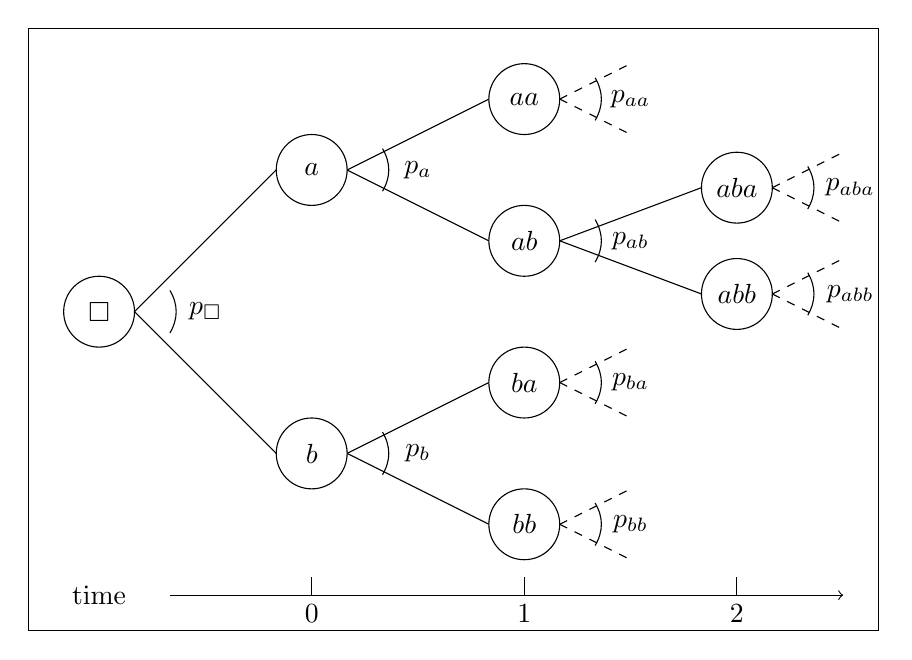
\begin{tikzpicture}[xscale=0.9,yscale=0.9]
%\draw[help lines] (-1,-0.5) grid (11,7.5);
\draw (-1,-1) rectangle (11,7.5);
\draw (0,3.5) circle(0.5) node[align=center] {$\Box$};
\draw (3,5.5) circle(0.5) node[align=center] {$a$};
\draw (3,1.5) circle(0.5) node[align=center] {$b$};
\draw (6,6.5) circle(0.5) node[align=center] {$aa$};
\draw (6,4.5) circle(0.5) node[align=center] {$ab$};
\draw (6,2.5) circle(0.5) node[align=center] {$ba$};
\draw (6,0.5) circle(0.5) node[align=center] {$bb$};
\draw (9,5.25) circle(0.5) node[align=center] {$aba$};
\draw (9,3.75) circle(0.5) node[align=center] {$abb$};
\draw (0.5,3.5) -- (2.5,5.5);
\draw (0.5,3.5) -- (2.5,1.5);
\draw (3.5,5.5) -- (5.5,6.5);
\draw (3.5,5.5) -- (5.5,4.5);
\draw (3.5,1.5) -- (5.5,2.5);
\draw (3.5,1.5) -- (5.5,0.5);
\draw (6.5,4.5) -- (8.5,5.25);
\draw (6.5,4.5) -- (8.5,3.75);
\draw [dashed] (6.5,6.5) -- (7.5,7);
\draw [dashed] (6.5,6.5) -- (7.5,6);
\draw [dashed] (6.5,2.5) -- (7.5,3);
\draw [dashed] (6.5,2.5) -- (7.5,2);
\draw [dashed] (6.5,0.5) -- (7.5,1);
\draw [dashed] (6.5,0.5) -- (7.5,0);
\draw [dashed] (9.5,5.25) -- (10.5,5.75);
\draw [dashed] (9.5,5.25) -- (10.5,4.75);
\draw [dashed] (9.5,3.75) -- (10.5,4.25);
\draw [dashed] (9.5,3.75) -- (10.5,3.25);
\draw (1.5,3.5) node[align=right] {$p_{\Box}$};
%\draw (1,3.8) .. controls (1.25,3.5) .. (1,3.2);
\draw (1,3.8) to[bend left] (1,3.2);
\draw (4.5,5.5) node[align=right] {$p_{a}$};
\draw (4,5.8) to[bend left] (4,5.2);
\draw (4.5,1.5) node[align=right] {$p_{b}$};
\draw (4,1.8) to[bend left] (4,1.2);
\draw (7.5,6.5) node[align=right] {$p_{aa}$};
\draw (7,6.8) to[bend left] (7,6.2);
\draw (7.5,4.5) node[align=right] {$p_{ab}$};
\draw (7,4.8) to[bend left] (7,4.2);
\draw (7.5,2.5) node[align=right] {$p_{ba}$};
\draw (7,2.8) to[bend left] (7,2.2);
\draw (7.5,0.5) node[align=right] {$p_{bb}$};
\draw (7,0.8) to[bend left] (7,0.2);
\draw (10.6,5.25) node[align=right] {$p_{aba}$};
\draw (10,5.55) to[bend left] (10,4.95);
\draw (10.6,3.75) node[align=right] {$p_{abb}$};
\draw (10,4.05) to[bend left] (10,3.45);
\draw (0,-0.5) node[align=center] {time};
\draw [->] (1,-0.5) -- (10.5,-0.5);
\draw (3,-0.5) -- (3,-0.25);
\draw (3, -0.5) node[align=center,below] {0};
\draw (6,-0.5) -- (6,-0.25);
\draw (6, -0.5) node[align=center,below] {1};
\draw (9,-0.5) -- (9,-0.25);
\draw (9, -0.5) node[align=center,below] {2};
\end{tikzpicture}
\caption{A (partial) event tree for a binary state-space $\states=\{a,b\}$. The vertices are situations, i.e. elements of $\states^*_\Box$, and edges are induced by the prefix order $\prec$. Dashed lines represent branches that are not shown in the figure. The tree has been augmented to a probability tree, by assigning to each $w\in\states^*$ a local model $p_w$. A time axis represents at which point in time the situations can occur.}
\label{fig:example_event_tree}
\end{figure}

Such an event tree can be turned into an intuitive representation of a stochastic process by augmenting it into a \emph{probability tree}. This is done by assigning to each situation $w\in\states^*_\Box$ in the tree a \emph{local model} $p_{w}$, which is a probability mass function on $\states$; that is, it is a map $p_w:\states\to\realsnonneg$ such that $\sum_{x\in\states}p_w(x)=1$. An example of this is again illustrated in Figure~\ref{fig:example_event_tree}.
\begin{definition}[Probability Tree]\label{def:prob_tree}
A probability tree is a tuple $(\states^*_\Box,\prec,p_{(\cdot)})$, where $\states^*_\Box$ is the set of all situations, $\prec$ is the prefix order on $\states^*_\Box$, and $p_{(\cdot)}:\states^*_\Box\times\states\to\realsnonneg$ represents all local models, so that $\sum_{x\in\states}p_w(x)=1$ for all $w\in\states^*_\Box$.
\end{definition}

The mechanism by which a stochastic process obtains a certain realisation $\omega\in\Omega$ can now be interpreted as performing a weighted, random walk along this probability tree, starting from $\Box$. Following the tree in Figure~\ref{fig:example_event_tree}, this is done as follows: from $\Box$, we transition either to $a$, with probability $p_\Box(a)$, or to $b$, with probability $p_\Box(b)$. Suppose we transition to $a$. From this new situation, the next step will take us either to $aa$, with probability $p_a(a)$, or to $ab$, with probability $p_a(b)$. Proceeding in this fashion, an infinite random walk along this tree generates a full path $\omega:\natswith\to\states$, where, for all $t\in\natswith$, the state $\omega(t)$ represents the (randomly chosen) branch that we took along the tree at the $(t+1)$-th step.

This ``path construction'' view allows us also to connect back to the measure-theoretic definition that we encountered earlier. To obtain this correspondence in one direction, fix a probability tree $(\states^*_\Box,\prec, p_{(\cdot)})$ and let $(\Omega,\mathcal{F})$ be an appropriate measurable space of discrete-time sample paths, on which we will aim to construct the measure $P$ quantifying in the measure-theoretic sense the uncertainty of the corresponding stochastic process $\{X_t\}_{t\in\natswith}$ on the resulting probability space.

We now reason intuitively by using the ``random walk'' along the probability tree. Starting from $\Box$, we transition to a first situation $x\in\states$ with probability $p_\Box(x)$. From there, we could then perform the entire infinite random walk to generate the remainder of the path. So, a different way of saying this is that, of all the random paths $\omega\in\Omega$ that could be generated, a fraction of $p_\Box(x)$ of them will start with $\omega(0)=x$. Using also the interpretation given by Corollary~\ref{cor:process_prob_is_measure}, it therefore makes sense to define the \emph{first-step marginal measure} $P^*(X_0=x) \coloneqq p_\Box(x)$ for all $x\in\states$.

Let us now consider the next step, and assume the first step down the tree resulted in a situation $x\in\states$. Then, with probability $p_x(y)$, $y\in\states$, the next situation will be $xy$. In terms of paths that could be generated, a fraction of $p_x(y)$ of the paths that satisfy $\omega(0)=x$, will furthermore satisfy $\omega(1)=y$. Therefore, we define for the \emph{second}-step marginal measure $P^*(X_0=x,X_1=y)\coloneqq p_\Box(x)p_x(y)$.

Proceeding in this manner, for every situation $w\in\states^*$ with length $n+1$, $n\in\natswith$, we can compute the $(n+1)$-th step marginal measure as
\begin{equation*}
P^*\bigl(X_{0:n}=w\bigr) \coloneqq p_\Box\bigl(w_0\bigr)\prod_{i=1}^{n} p_{w_0\cdots w_{i-1}}\bigl(w_i\bigr)\,,
\end{equation*}
or in words, by multiplying all probabilities given by the local models of the situations encountered on the path from the root of the tree, down to the situation $w$.

A fundamental result in the measure-theoretic treatment of stochastic processes (known as the \emph{Kolmogorov extension theorem}) states that the collection of all these $n$-th step marginal measures $P^*$ induces (``coherently'') a probability measure $P$ on $(\Omega,\mathcal{F})$. Specifically, the finite $n$-th step marginals of $P$ will correspond exactly to these $n$-th step marginal measures that we constructed from the probability tree. This establishes the connection between probability trees and discrete-time measure-theoretic stochastic processes, in that the latter can be constructed from the former.

For the other direction, so, to construct a probability tree from a given probability space $(\Omega,\mathcal{F},P)$, we start with an event tree $(\states^*_\Box,\prec)$ and aim to construct the local models $p_{(\cdot)}$. Using the intuitive interpretation offered by Corollary~\ref{cor:process_prob_is_measure}, we start by setting $p_\Box(x)=P(X_0=x)$ for all $x\in\states$. For all other situations $w\in\states^*$ with length $n+1$, $n\in\natswith$, the local model $p_w$ is defined as the conditional measure constructed from Bayes' rule, i.e., for all $x\in\states$,
\begin{align}\label{eq:local_prob_tree_from_measure}
p_w(x) &= P\bigl( X_{n+1}=x\,\big\vert\, X_{0:n}=w \bigr) = \frac{P\bigl(X_{0:n}=w, X_{n+1}=x\bigr)}{P\bigl( X_{0:n}=w \bigr)}\,.
\end{align}
This also establishes the connection in the other direction. It can be verified that, by now constructing from this probability tree a measure $P^*$, say, in the manner described above, we obtain again $P^*=P$; so, we conclude that this yields a one-to-one correspondence between probability trees and measure-theoretic stochastic processes.

It should be noted that the second direction in the preceding discussion has one (rather large) caveat: it does not work when there are partial paths that have zero probability to occur. This is because then Bayes' rule cannot define the conditional measure required to construct the local model for the situation corresponding to that partial path, since it would result in a division by zero.

To summarise, we can conclude that there is indeed a correspondence between the two representations that we have seen so far (up to some technical difficulties surrounding probabilities that are zero). We have seen that the graphical tree structure allows us to reason intuitively about how a stochastic process generates a sample path, by ``walking'' from the root of the tree down its branches. As we will discuss next, we can also use this structure to ``reason backwards'': from vertices deep down in the tree back to the root. We will see that this allows one to intuitively derive \emph{computational methods} for working with stochastic processes. 

So, fix $n\in\natswith$ and let $f\in\gambles(\states^{n+1})$ be a real-valued function of which we aim to compute the expected value with respect to the random variables $X_{0:n}$ at the time points $0,\ldots,n\in\natswith$. Note that it suffices to consider this case, in the sense that any function defined on a subset of the variables $X_{0:n}$, can always be trivially extended to a function on all of them. Now first notice the following. For any situation $w\in\states^*$ with length $\lvert w\rvert = n+1$, the value of $f$ in $w$ is easy to compute; it is simply $f(w)$. Hence in particular, the \emph{expected value} of $f$, in $w$, is simply
\begin{equation*}
\mathbb{E}\bigl[f(X_{0:n})\,\big\vert\,X_{0:n}=w\bigr] = f(w)\,.
\end{equation*}
Recall that the situation $w$ represents a node in the event tree. We will now ``pull back'' the above expected value, to the time-point $n-1$. Consider therefore the parent situation of $w$ in the probability tree; we will compute the expected value of $f$ in this parent situation.

This parent is a situation $v$ of length $\lvert v\lvert=\lvert w\lvert-1=n$, which entirely coincides with $w$: $v_i=w_i$ for all $i=0,\ldots,n-1$. Associated to $v$ is the local probability model $p_v$ which, as we have discussed above, represents the probability with which a random walk along the tree travels through the various children of $v$. In particular, such a random walk goes through the situation $w$, with probability $p_v(w_\top)$. Therefore, the contribution of the expected value in $w$, to the expected value in $v$, is the expected value in $w$ weighted by $p_v(w_\top)$. Since this holds for all children of $v$, we can write
\begin{align*}
&\mathbb{E}\bigl[f(X_{0:n}) \,\big\vert\, X_{0:(n-1)}=v \bigr] = \sum_{x\in\states} p_v(x)\mathbb{E}\bigl[f(X_{0:n})\,\big\vert\,X_{0:(n-1)}=v,X_n=x\bigr]\,.
\end{align*}
This ``pullback'' operation is graphically illustrated in Figure~\ref{fig:pullback_loie}.

\begin{figure}
\centering
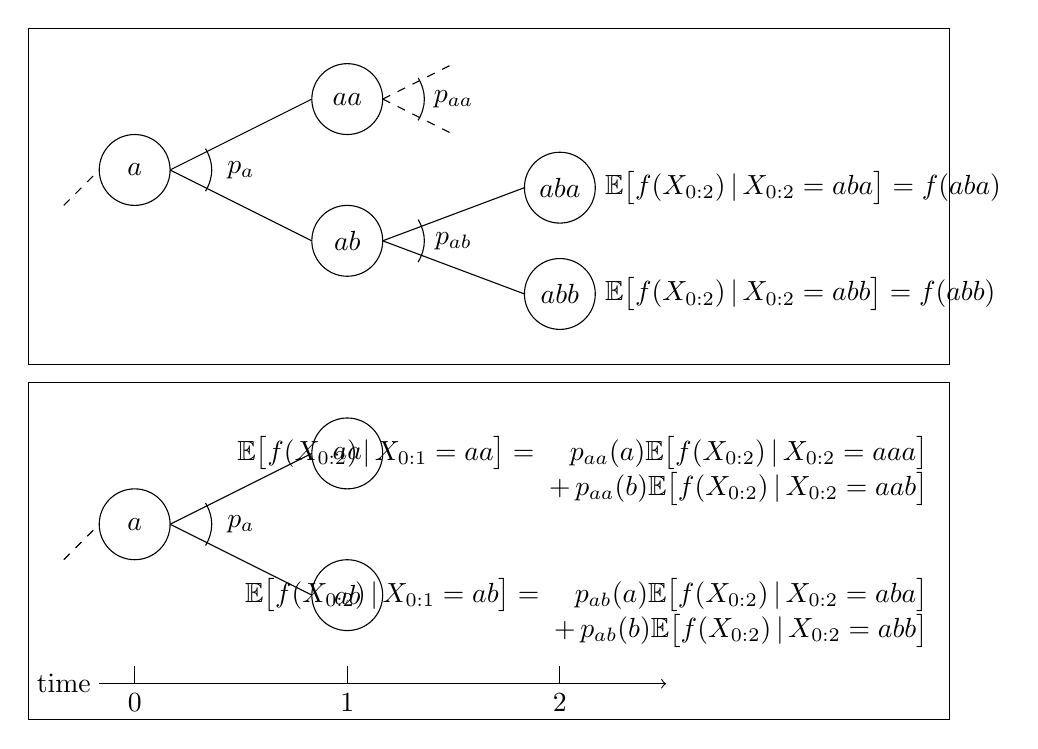
\begin{tikzpicture}[xscale=0.9,yscale=0.9]
%\draw[help lines] (-1,-0.5) grid (11,7.5);
\draw (-0.5,2.75) rectangle (12.5,7.5);
\draw (1,5.5) circle(0.5) node[align=center] {$a$};
\draw (4,6.5) circle(0.5) node[align=center] {$aa$};
\draw (4,4.5) circle(0.5) node[align=center] {$ab$};
\draw (7,5.25) circle(0.5) node[align=center] {$aba$};
\draw (7,3.75) circle(0.5) node[align=center] {$abb$};
\draw [dashed] (0,5) -- (0.5,5.5);
\draw (1.5,5.5) -- (3.5,6.5);
\draw (1.5,5.5) -- (3.5,4.5);
\draw (4.5,4.5) -- (6.5,5.25);
\draw (4.5,4.5) -- (6.5,3.75);
\draw [dashed] (4.5,6.5) -- (5.5,7);
\draw [dashed] (4.5,6.5) -- (5.5,6);
\draw (2.5,5.5) node[align=right] {$p_{a}$};
\draw (2,5.8) to[bend left] (2,5.2);
\draw (5.5,6.5) node[align=right] {$p_{aa}$};
\draw (5,6.8) to[bend left] (5,6.2);
\draw (5.5,4.5) node[align=right] {$p_{ab}$};
\draw (5,4.8) to[bend left] (5,4.2);
\draw (7.5,5.25) node[anchor=west] {$\mathbb{E}\bigl[f(X_{0:2})\,\vert\,X_{0:2}=aba\bigr]=f(aba)$};
\draw (7.5,3.75) node[anchor=west] {$\mathbb{E}\bigl[f(X_{0:2})\,\vert\,X_{0:2}=abb\bigr]=f(abb)$};
%
%
\draw (-0.5,-2.25) rectangle (12.5,2.5);
\draw (1,0.5) circle(0.5) node[align=center] {$a$};
\draw (4,1.5) circle(0.5) node[align=center] {$aa$};
\draw (4,-0.5) circle(0.5) node[align=center] {$ab$};
\draw [dashed] (0,0) -- (0.5,0.5);
\draw (1.5,0.5) -- (3.5,1.5);
\draw (1.5,0.5) -- (3.5,-0.5);
\draw (2.5,0.5) node[align=right] {$p_{a}$};
\draw (2,0.8) to[bend left] (2,0.2);
%\draw (4.5,1.5) node[anchor=west] {$\mathbb{E}\bigl[f(X_{0:2})\,\vert\,X_{0:1}=aa\bigr]$};
\draw (12.33,1.5) node[anchor=east] {$\mathbb{E}\bigl[f(X_{0:2})\,\vert\,X_{0:1}=aa\bigr]= \quad p_{aa}(a)\mathbb{E}\bigl[f(X_{0:2})\,\vert\,X_{0:2}=aaa\bigr]$};
\draw (12.33,1) node[anchor=east] {$+\,  p_{aa}(b)\mathbb{E}\bigl[f(X_{0:2})\,\vert\,X_{0:2}=aab\bigr]$};
\draw (12.33,-0.5) node[anchor=east] {$\mathbb{E}\bigl[f(X_{0:2})\,\vert\,X_{0:1}=ab\bigr]= \quad p_{ab}(a)\mathbb{E}\bigl[f(X_{0:2})\,\vert\,X_{0:2}=aba\bigr]$};
\draw (12.33,-1) node[anchor=east] {$+\,  p_{ab}(b)\mathbb{E}\bigl[f(X_{0:2})\,\vert\,X_{0:2}=abb\bigr]$};
%\draw (4.62,2.5) -- (4.62,-1.5);
\draw (0,-1.75) node[align=center] {time};
\draw [->] (0.5,-1.75) -- (8.5,-1.75);
\draw (1,-1.75) -- (1,-1.5);
\draw (1, -1.75) node[align=center,below] {0};
\draw (4,-1.75) -- (4,-1.5);
\draw (4, -1.75) node[align=center,below] {1};
\draw (7,-1.75) -- (7,-1.5);
\draw (7, -1.75) node[align=center,below] {2};
\end{tikzpicture}
\caption{Graphical illustration of ``pulling back'' the expected value of a function $f$ on $X_{0:2}$, in a probability tree on a binary state-space $\states=\{a,b\}$. Top: the function $f$ is entirely determined by the situations of length 3, i.e. the expected value of the function in those situations, is simply the value of the function evaluated in that situation. Bottom: result after ``pulling back'' the expectations by one step. The resulting conditional expectation is a function whose value is entirely determined by the situations of length 2. The values are the weighted average of the expectations in the child nodes, weighted by the local models $p_{(\cdot)}$.}
\label{fig:pullback_loie}
\end{figure}

Now, observe that the above conditional expectation of $f$ in $v$, is itself a real-valued function in $\gambles(\states^n)$. Its value is determined by the states at times $0,\ldots,n-1$. We can therefore repeat the above argument; we pull back to the parent of $v$, then to the parent of \emph{that} situation, and so on. Eventually, the parent that we are considering is the empty situation $\Box$; we then finish by computing
\begin{equation*}
\mathbb{E}\bigl[f(X_{0:n})\bigr] = \sum_{x\in\states} p_\Box(x) \mathbb{E}\bigl[f(X_{0:n})\,\big\vert\,X_0=x\bigr]\,,
\end{equation*}
which is exactly the expected value of $f$ that we started out wanting to compute.

This method to compute the expected value of a function by ``pulling back'' the ``local'', or conditional, expected values, uses the interpretation of a stochastic process as a probability tree. The method relies on a property that is called the \emph{law of iterated expectation}, or alternatively the \emph{law of total probability}. It can be stated formally in the measure-theoretic context, where it is also easily stated for \emph{continuous}-time stochastic processes.
\begin{theorem}\label{thm:loie}
Fix a time-dimension $\timedim\in\{\natswith,\realsnonneg\}$, and let $\{X_t\}_{t\in\timedim}$ be a stochastic process on $(\Omega,\mathcal{F},P)$. Choose any three ordered sequences $\mathbf{s}=s_1,\ldots,s_n$, $\mathbf{t}=t_1,\ldots,t_m$, and $\mathbf{u}=u_1,\ldots,u_\ell$ in $\timedim$, with $n,m,\ell\in\nats$ such that $s_n<t_1$ and $t_m<u_1$. Then for any real-valued function $f\in\gambles(\states^{n+m+\ell})$ on $X_\mathbf{s},X_\mathbf{t},X_\mathbf{u}$, it holds that
\begin{equation*}
\mathbb{E}\bigl[f(X_\mathbf{s},X_\mathbf{t},X_\mathbf{u})\,\big\vert\,X_\mathbf{s}\bigr] = \mathbb{E}\Bigl[\mathbb{E}\bigl[f(X_\mathbf{s},X_\mathbf{t},X_\mathbf{u})\,\big\vert\,X_\mathbf{s},X_\mathbf{t}\bigr]\,\Big\vert\,X_\mathbf{s}\Bigr]\,,
\end{equation*} 
whenever $P(X_\mathbf{s})$ and $P(X_\mathbf{s},X_\mathbf{t})$ are everywhere strictly positive.
\end{theorem}

Having discussed how to interpret probability trees, and how to use them to reason about the computation of expected values, we now move on to a discussion of their structural properties. Note that the specification of a probability tree is still relatively complicated. This is not really due to the structure of the tree; the situations $\states^*_\Box$ and prefix order $\prec$ carry enough information to construct the tree up to any desired level, and their mathematical specification is straightforward. However, in order to specify all the local models $p_{(\cdot)}$, we need to provide an infinite number of probability mass functions on $\states$; one for each situation $w\in\states^*_\Box$. This is why one often restricts attention to simpler models, where one needs less, and often only finitely many, local models.

These simplifications can be seen as a matter of degree. At the one extreme, we have the general definition that we used above, where each situation $w\in\states^*_\Box$ has a local model $p_w$. This leads to a lot of possible structure, but is hard to specify. At the other extreme is the \emph{independent and identically distributed} (i.i.d.) process; this is when we only have a single probability mass function $p$, and we set $p_w\coloneqq p$ for all $w\in\states^*_\Box$. For such a process, no matter what situation we are in, the next branch will always be chosen according to $p$. This process is easy to specify, but it does not yield a lot of structure that can capture the dynamics of the underlying system that we are trying to model.

A useful step up from the i.i.d. process is reached by the popular class of models known as \emph{homogeneous Markov chains}. For a homogeneous Markov chain, the local model \emph{only} depends on the last step of the corresponding situation, and not on what happened before that:
\begin{definition}[Homogeneous Markov Chain as Probability Tree]\label{def:prob_tree_homogen_markov}
A probability tree $(\states^*_\Box,\prec,p_{(\cdot)})$ is called a homogeneous Markov chain if, for all situations $v,w\in\states^*$ such that $v_\top=w_\top$, it holds that $p_v=p_w$.
\end{definition} 
\begin{corollary}
Let $(\states^*_\Box,\prec,p_{(\cdot)})$ be a homogeneous Markov chain. Then for all $x\in\states$ and all $w\in\states^*$ such that $w_\top=x$, it holds that $p_w=p_x$.
\end{corollary}
\begin{proof}
Trivial from Definition~\ref{def:prob_tree_homogen_markov} and the fact that all $x\in\states$ are also situations. 
\end{proof}
\begin{figure}
\centering
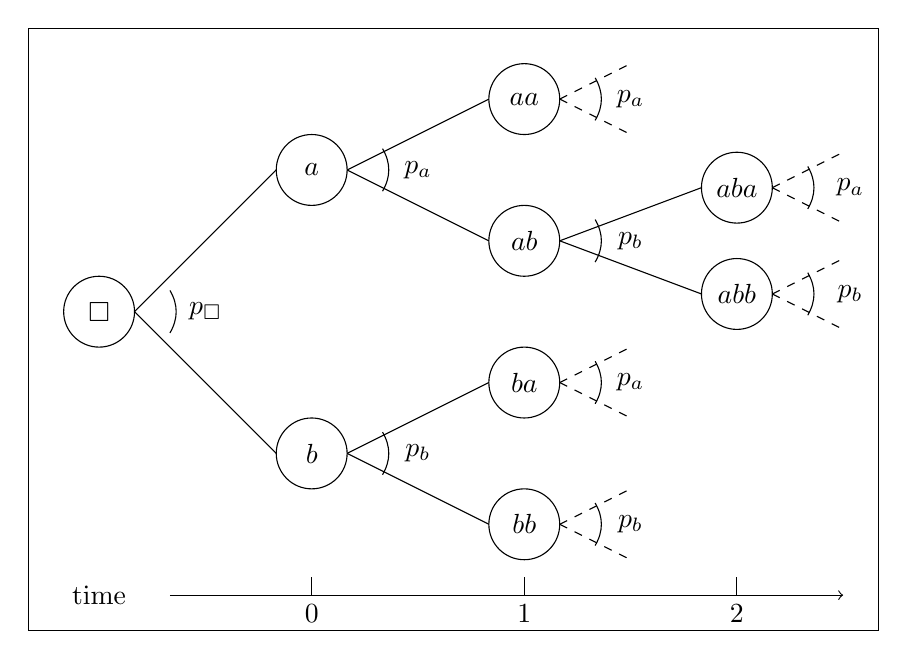
\begin{tikzpicture}[xscale=0.9,yscale=0.9]
%\draw[help lines] (-1,-0.5) grid (11,7.5);
\draw (-1,-1) rectangle (11,7.5);
\draw (0,3.5) circle(0.5) node[align=center] {$\Box$};
\draw (3,5.5) circle(0.5) node[align=center] {$a$};
\draw (3,1.5) circle(0.5) node[align=center] {$b$};
\draw (6,6.5) circle(0.5) node[align=center] {$aa$};
\draw (6,4.5) circle(0.5) node[align=center] {$ab$};
\draw (6,2.5) circle(0.5) node[align=center] {$ba$};
\draw (6,0.5) circle(0.5) node[align=center] {$bb$};
\draw (9,5.25) circle(0.5) node[align=center] {$aba$};
\draw (9,3.75) circle(0.5) node[align=center] {$abb$};
\draw (0.5,3.5) -- (2.5,5.5);
\draw (0.5,3.5) -- (2.5,1.5);
\draw (3.5,5.5) -- (5.5,6.5);
\draw (3.5,5.5) -- (5.5,4.5);
\draw (3.5,1.5) -- (5.5,2.5);
\draw (3.5,1.5) -- (5.5,0.5);
\draw (6.5,4.5) -- (8.5,5.25);
\draw (6.5,4.5) -- (8.5,3.75);
\draw [dashed] (6.5,6.5) -- (7.5,7);
\draw [dashed] (6.5,6.5) -- (7.5,6);
\draw [dashed] (6.5,2.5) -- (7.5,3);
\draw [dashed] (6.5,2.5) -- (7.5,2);
\draw [dashed] (6.5,0.5) -- (7.5,1);
\draw [dashed] (6.5,0.5) -- (7.5,0);
\draw [dashed] (9.5,5.25) -- (10.5,5.75);
\draw [dashed] (9.5,5.25) -- (10.5,4.75);
\draw [dashed] (9.5,3.75) -- (10.5,4.25);
\draw [dashed] (9.5,3.75) -- (10.5,3.25);
\draw (1.5,3.5) node[align=right] {$p_{\Box}$};
%\draw (1,3.8) .. controls (1.25,3.5) .. (1,3.2);
\draw (1,3.8) to[bend left] (1,3.2);
\draw (4.5,5.5) node[align=right] {$p_{a}$};
\draw (4,5.8) to[bend left] (4,5.2);
\draw (4.5,1.5) node[align=right] {$p_{b}$};
\draw (4,1.8) to[bend left] (4,1.2);
\draw (7.5,6.5) node[align=right] {$p_{a}$};
\draw (7,6.8) to[bend left] (7,6.2);
\draw (7.5,4.5) node[align=right] {$p_{b}$};
\draw (7,4.8) to[bend left] (7,4.2);
\draw (7.5,2.5) node[align=right] {$p_{a}$};
\draw (7,2.8) to[bend left] (7,2.2);
\draw (7.5,0.5) node[align=right] {$p_{b}$};
\draw (7,0.8) to[bend left] (7,0.2);
\draw (10.6,5.25) node[align=right] {$p_{a}$};
\draw (10,5.55) to[bend left] (10,4.95);
\draw (10.6,3.75) node[align=right] {$p_{b}$};
\draw (10,4.05) to[bend left] (10,3.45);
\draw (0,-0.5) node[align=center] {time};
\draw [->] (1,-0.5) -- (10.5,-0.5);
\draw (3,-0.5) -- (3,-0.25);
\draw (3, -0.5) node[align=center,below] {0};
\draw (6,-0.5) -- (6,-0.25);
\draw (6, -0.5) node[align=center,below] {1};
\draw (9,-0.5) -- (9,-0.25);
\draw (9, -0.5) node[align=center,below] {2};
\end{tikzpicture}
\caption{A homogeneous Markov chain, represented as a probability tree.}
\label{fig:example_homogen_markov_tree}
\end{figure}
An example for the binary state space $\states=\{a,b\}$ is shown in Figure~\ref{fig:example_homogen_markov_tree}. Additional degrees of freedom can be introduced back into this model by also letting the local models depend on the corresponding depth of the tree. The dynamics can then depend on the point in time, but not on the \emph{specific} history up to that time. This yields the more general definition of a (non-homogeneous) \emph{Markov chain}:
\begin{definition}[Markov Chain as Probability Tree]\label{def:prob_tree_markov}
A probability tree $(\states^*_\Box,\prec,p_{(\cdot)})$ is called a Markov chain if, for all situations $v,w\in\states^*$ for which $\lvert v\rvert=\lvert w\rvert$ and $v_\top=w_\top$, it holds that $p_v=p_w$.
\end{definition}
\begin{figure}
\centering
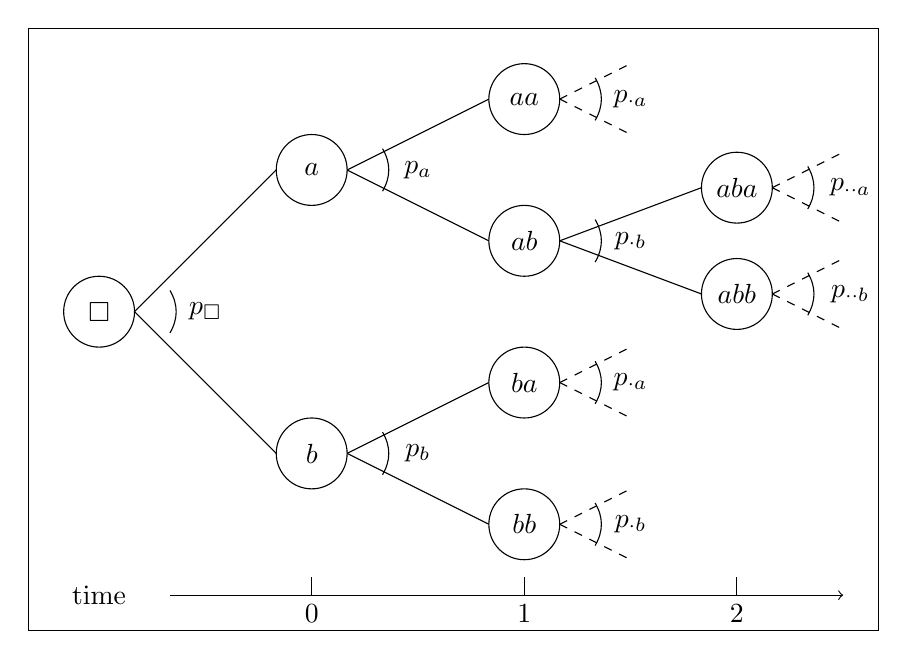
\begin{tikzpicture}[xscale=0.9,yscale=0.9]
%\draw[help lines] (-1,-0.5) grid (11,7.5);
\draw (-1,-1) rectangle (11,7.5);
\draw (0,3.5) circle(0.5) node[align=center] {$\Box$};
\draw (3,5.5) circle(0.5) node[align=center] {$a$};
\draw (3,1.5) circle(0.5) node[align=center] {$b$};
\draw (6,6.5) circle(0.5) node[align=center] {$aa$};
\draw (6,4.5) circle(0.5) node[align=center] {$ab$};
\draw (6,2.5) circle(0.5) node[align=center] {$ba$};
\draw (6,0.5) circle(0.5) node[align=center] {$bb$};
\draw (9,5.25) circle(0.5) node[align=center] {$aba$};
\draw (9,3.75) circle(0.5) node[align=center] {$abb$};
\draw (0.5,3.5) -- (2.5,5.5);
\draw (0.5,3.5) -- (2.5,1.5);
\draw (3.5,5.5) -- (5.5,6.5);
\draw (3.5,5.5) -- (5.5,4.5);
\draw (3.5,1.5) -- (5.5,2.5);
\draw (3.5,1.5) -- (5.5,0.5);
\draw (6.5,4.5) -- (8.5,5.25);
\draw (6.5,4.5) -- (8.5,3.75);
\draw [dashed] (6.5,6.5) -- (7.5,7);
\draw [dashed] (6.5,6.5) -- (7.5,6);
\draw [dashed] (6.5,2.5) -- (7.5,3);
\draw [dashed] (6.5,2.5) -- (7.5,2);
\draw [dashed] (6.5,0.5) -- (7.5,1);
\draw [dashed] (6.5,0.5) -- (7.5,0);
\draw [dashed] (9.5,5.25) -- (10.5,5.75);
\draw [dashed] (9.5,5.25) -- (10.5,4.75);
\draw [dashed] (9.5,3.75) -- (10.5,4.25);
\draw [dashed] (9.5,3.75) -- (10.5,3.25);
\draw (1.5,3.5) node[align=right] {$p_{\Box}$};
%\draw (1,3.8) .. controls (1.25,3.5) .. (1,3.2);
\draw (1,3.8) to[bend left] (1,3.2);
\draw (4.5,5.5) node[align=right] {$p_{a}$};
\draw (4,5.8) to[bend left] (4,5.2);
\draw (4.5,1.5) node[align=right] {$p_{b}$};
\draw (4,1.8) to[bend left] (4,1.2);
\draw (7.5,6.5) node[align=right] {$p_{\cdot a}$};
\draw (7,6.8) to[bend left] (7,6.2);
\draw (7.5,4.5) node[align=right] {$p_{\cdot b}$};
\draw (7,4.8) to[bend left] (7,4.2);
\draw (7.5,2.5) node[align=right] {$p_{\cdot a}$};
\draw (7,2.8) to[bend left] (7,2.2);
\draw (7.5,0.5) node[align=right] {$p_{\cdot b}$};
\draw (7,0.8) to[bend left] (7,0.2);
\draw (10.6,5.25) node[align=right] {$p_{\cdot\cdot a}$};
\draw (10,5.55) to[bend left] (10,4.95);
\draw (10.6,3.75) node[align=right] {$p_{\cdot\cdot b}$};
\draw (10,4.05) to[bend left] (10,3.45);
\draw (0,-0.5) node[align=center] {time};
\draw [->] (1,-0.5) -- (10.5,-0.5);
\draw (3,-0.5) -- (3,-0.25);
\draw (3, -0.5) node[align=center,below] {0};
\draw (6,-0.5) -- (6,-0.25);
\draw (6, -0.5) node[align=center,below] {1};
\draw (9,-0.5) -- (9,-0.25);
\draw (9, -0.5) node[align=center,below] {2};
\end{tikzpicture}
\caption{A (non-homogeneous) Markov chain, represented as a probability tree.}
\label{fig:example_markov_tree}
\end{figure}
An example for the binary state space $\states=\{a,b\}$ is shown in Figure~\ref{fig:example_markov_tree}. It can be verified that a homogeneous Markov chain is a Markov chain, but not---in general---the other way around. 
Note that, in contrast to homogeneous Markov chains where we only needed to specify local models $p_x$ for all $x\in\states$, we now need different local models for each level of the tree. So, we are now back to needing an infinite number of local models in order to fully describe such a model.

These definitions of (homogeneous) Markov chains can also be conveniently translated back to the measure-theoretic context. We here give the general definition, for an arbitrary time-dimension (so, either $\timedim=\natswith$ or $\timedim=\realsnonneg$) and multiple steps into the future:
\begin{definition}[Markov Chain as Probability Measure]\label{def:measure_markov}
A stochastic process $\{X_t\}_{t\in\timedim}$ on $(\Omega,\mathcal{F},P)$ is called a Markov chain if for all $s_1,\ldots,s_n,t\in\timedim$, $n\in\nats$, such that $s_1<\cdots<s_n<t$, it holds that $P(X_t\,\vert\,X_{s_1},\ldots,X_{s_n}) = P(X_t\,\vert\,X_{s_n})$. A stochastic process that is a Markov chain, is said to have the Markov property.
\end{definition}
Similarly, the notion of homogeneity can be defined measure-theoretically and for an arbitrary time-dimension:  
\begin{definition}[Homogeneous Markov Chain as Probability Measure]\label{def:measure_homogen_markov}
A stochastic process $\{X_t\}_{t\in\timedim}$ on $(\Omega,\mathcal{F},P)$ is called a homogeneous Markov chain if it is a Markov chain, and if additionally, for all $s,t\in\timedim$ such that $s<t$, it holds that $P(X_t\,\vert\,X_s)=P(X_{t-s}\,\vert\,X_0)$.
\end{definition}
We leave it as an exercise to verify that, when $\timedim=\natswith$, Definitions~\ref{def:measure_markov} and~\ref{def:measure_homogen_markov} correspond to what we would expect from Definitions~\ref{def:prob_tree_markov} and~\ref{def:prob_tree_homogen_markov}, respectively.

\subsection{Probabilistic Graphical Models}\label{sec:pgm}

We now move on to a different graphical representation of stochastic processes, that is useful for Markov chains in particular: \emph{probabilistic graphical models} (PGMs), which are also known as \emph{Bayesian networks}. While the graphical structure of probability trees in Section~\ref{sec:prob_trees} emphasised the partial paths in the realisation of a stochastic process, the PGM representation emphasises the individual random variables $X_t$. 

The PGM representation of a discrete-time Markov chain $\{X_t\}_{t\in\natswith}$ is given in Figure~\ref{fig:example_markov_pgm}. The structure is a directed acyclic graph, with one node associated to each random variable $X_t$, and arcs representing the dependence of the receiving node's random variable's distribution, on the originating node's random variable's value. Due to the Markov property (c.f. Definition~\ref{def:measure_markov}), each random variable $X_n$, $n\in\nats$, is only (``directly'') dependent on $X_{n-1}$, the value of the random variable immediately before it. The initial variable $X_0$ is somewhat of a special case, since it does not depend on any other variables; there are no time-points preceding it. Due to these properties, the graphical structure is that of a chain; this may go some way in explaining the name ``Markov chain''. In the remainder of this section, we will refer to both a node in the PGM and to its random variable, using the notation $X_t$.
\begin{figure}
\centering
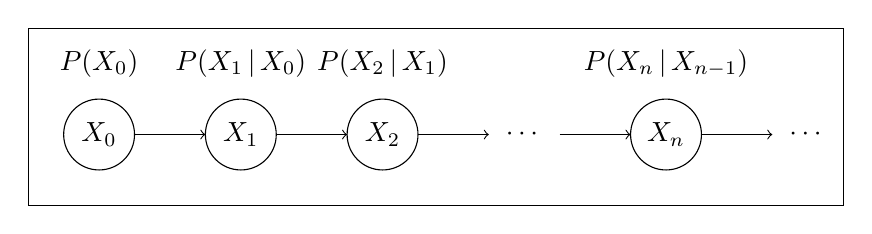
\begin{tikzpicture}[xscale=0.9,yscale=0.9]
%\draw[help lines] (-1,-0.5) grid (11,7.5);
\draw (-1,-1) rectangle (10.5,1.5);
\draw (0,0) circle(0.5) node[align=center] {$X_0$};
\draw (0,1) node[align=right] {$P(X_0)$};
\draw [->] (0.5,0) -- (1.5,0);
\draw (2,0) circle(0.5) node[align=center] {$X_1$};
\draw (2,1) node[align=right] {$P(X_1\,\vert\,X_0)$};
\draw [->] (2.5,0) -- (3.5,0);
\draw (4,0) circle(0.5) node[align=center] {$X_2$};
\draw (4,1) node[align=right] {$P(X_2\,\vert\,X_1)$};
\draw [->] (4.5,0) -- (5.5,0);
\draw (6,0) node[align=right] {$\cdots$};
\draw [->] (6.5,0) -- (7.5,0);
\draw (8,0) circle(0.5) node[align=center] {$X_n$};
\draw (8,1) node[align=right] {$P(X_n\,\vert\,X_{n-1})$};
\draw [->] (8.5,0) -- (9.5,0);
\draw (10,0) node[align=right] {$\cdots$};
\end{tikzpicture}
\caption{Probabilistic graphical model representation of a discrete-time Markov chain $\{X_t\}_{t\in\natswith}$. Nodes represent random variables. An incoming arc on a node represents that the distribution of the corresponding random variable is influenced by the originating node of that arc. Correspondingly, each node associates a probability distribution to its random variable, conditional on the values of the random variables of the nodes on which it is dependent.}
\label{fig:example_markov_pgm}
\end{figure}

It should be emphasised that the graphical structure is not saying that only nodes which are adjacent in the PGM can influence each other. The formal interpretation is as follows: for any node $X_n$, $n\in\nats$, \emph{conditional on the value of the parent(s) of $X_n$}, the distribution of $X_n$ is probabilistically independent of the non-parents, non-descendants of $X_n$. This is the general interpretation of the independence properties of the arcs in a PGM. In the special case of Markov chains that we are considering here, the interpretation vastly simplifies. Notably, the ``non-parents, non-descendants'' of any node $X_n$ are exactly its ``grand-parents'', ``great-grand-parents'', and so on; it is the set of nodes $\{X_{m}\,:\,m\in\natswith,\, m<n-1\}$.

Put differently, the value of $X_n$ influences the distribution of \emph{all} of its descendants (i.e. the nodes $X_m$, $m>n$), so long as we do not know the value of any of those descendants themselves. We will next consider how to can quantify this.

We start by observing that for each node $X_n$, $n\in\nats$, we have the associated conditional probability $P(X_n\,\vert\,X_{n-1})$. Since the state-space $\states$ is taken to be finite, we can conveniently represent these conditional probabilities in a $\lvert\states\rvert\times\lvert\states\rvert$ matrix. For any $t\in\natswith$, this matrix $T_t$ is defined, for all $x,y\in\states$, as
\begin{equation}\label{eq:trans_mat_from_measure}
T_t(x,y) \coloneqq P(X_{t+1}=y\,\vert\,X_t=x)\,,
\end{equation}
where the indexing is taken to be row-first. This matrix $T_t$ is called the \emph{transition matrix} of the Markov chain at time $t$. Its elements $T_t(x,y)$ are called the \emph{transition probabilities from $x$ to $y$}, and they are the probabilities that a system that is in state $x$ at time $t$, will be in state $y$ at time $t+1$. This explains the subscript-indexing, whereby the matrix $T_t$ contains the conditional probabilities associated to node $X_{t+1}$.

These transition matrices make it easy to connect back to the probability tree representation of Markov chains that we encountered earlier:
\begin{proposition}
Let $(\states^*_\Box,\prec,p_{(\cdot)})$ be a probability tree that is a Markov chain, and let $T_t$ denote the associated family of transition matrices, as defined above. Then for all $t\in\nats$ and all $w\in\states^*$ such that $\lvert w\rvert = t$, it holds that $p_w(y)=T_t(w_\top, y)$ for all $y\in\states$.
\end{proposition}
\begin{proof}
Use Equation~\eqref{eq:local_prob_tree_from_measure}, Definition~\ref{def:measure_markov}, and Equation~\eqref{eq:trans_mat_from_measure}.
\end{proof}

The reason that we represent these probabilities using matrices is that this opens up the entire toolbox of linear algebra. We will see that this allows us to very succinctly write down certain relations and properties. For instance, we can now write the influence of a node on its descendants, using a simple matrix product:
\begin{proposition}\label{prop:markov_factor_transmat}
Let $\{X_t\}_{t\in\natswith}$ be a discrete-time Markov chain, and let $T_t$ be the associated family of transition matrices, as defined above. Then for all $s,t\in\natswith$ such that $s\leq t$, and all $x,y\in\states$, it holds that $P(X_{t+1}=y\,\vert\,X_s=x) = \left[T_s\cdots T_{t}\right](x,y)$.
\end{proposition}
\begin{proof}
We give a proof by induction. For $t=s$ the result is immediate from the definition of the transition matrix $T_s$. Now suppose the result is true for $t-1$; we show that it is also true for $t$:
\begin{align*}
P(X_{t+1}=y\,\vert\,X_s=x) &= \sum_{z\in\states} P(X_{t+1}=y,X_{t}=z\,\vert\,X_s=x) \\
 &= \sum_{z\in\states} P(X_{t}=z\,\vert\,X_s=x) P(X_{t+1}=y\,\vert\,X_{t}=z,\,X_s=x) \\
 &= \sum_{z\in\states} \left[T_s\cdots T_{t-1}\right](x,z) P(X_{t+1}=y\,\vert\,X_{t}=z) \\
 &= \sum_{z\in\states} \left[T_s\cdots T_{t-1}\right](x,z) T_{t}(z,y) = \bigl[T_s\cdots T_{t-1}T_{t}\bigr](x,y)\,,
\end{align*}
where the first and second equalities are basic properties of probabilities, the third equality is due to the induction hypothesis and the Markov property (c.f. Definition~\ref{def:measure_markov}), the fourth equality uses the definition of the transition matrix $T_{t}$, and the final equality uses the definition of a matrix product. 
\end{proof}

Another useful property of this representation, is that it allows us to write conditional expectations of functions $f\in\gamblesX$ using matrix-vector products. In particular, again because $\states$ is finite, any $f\in\gamblesX$ can be interpreted as a vector in $\reals^{\lvert\states\rvert}$; the coordinates are simply the values $f(x)$, $x\in\states$. Hence:
\begin{proposition}\label{prop:expectation_using_transmat}
Let $\{X_t\}_{t\in\natswith}$ be a discrete-time Markov chain, and let $T_t$ be the associated family of transition matrices. Then, for all $f\in\gamblesX$, all $t\in\natswith$, and all $x\in\states$, it holds that $\mathbb{E}\bigl[f(X_{t+1})\,\vert\,X_t=x\bigr] = \left[T_tf\right](x)$.
\end{proposition}
\begin{proof}
Simply use the definition of the matrix-vector product: 
\begin{equation*}
\left[T_tf\right](x)=\sum_{y\in\states}T_t(x,y)f(y)=\sum_{y\in\states}P(X_{t+1}=y\,\vert\,X_t=x)f(y) = \mathbb{E}\bigl[f(X_{t+1})\,\vert\,X_t=x\bigr].
\vspace{-16pt}
\end{equation*}
\end{proof}

The above properties can be combined to give a simplified version of the law of iterated expectation (Theorem~\ref{thm:loie}) that we encountered in Section~\ref{sec:prob_trees}:
\begin{corollary}\label{cor:trans_mat_loie}
Let $\{X_t\}_{t\in\natswith}$ be a discrete-time Markov chain, and let $T_t$ be the associated family of transition matrices. Then, for all $f\in\gamblesX$, all $s,t\in\natswith$ such that $s\leq t$, and all $x\in\states$, it holds that $\mathbb{E}\bigl[f(X_{t+1})\,\vert\,X_s=x\bigr] = \left[T_s\cdots T_tf\right](x)$.
\end{corollary}
\begin{proof}
Immediate from Propositions~\ref{prop:markov_factor_transmat} and~\ref{prop:expectation_using_transmat}.
\end{proof}
Note that, where the law of iterated expectation in Theorem~\ref{thm:loie} could be interpreted as ``pulling back'' in the associated probability tree, the above simplified version can additionally be interpreted as ``pulling back'' the conditional expectations in the associated PGM, through the product of the transition matrices. This is graphically represented in Figure~\ref{fig:example_loie_pgm}.
\begin{figure}
\centering
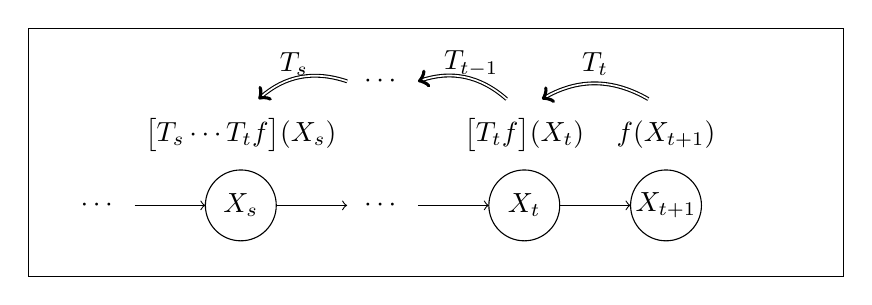
\begin{tikzpicture}[xscale=0.9,yscale=0.9]
%\draw[help lines] (-1,-0.5) grid (11,7.5);
\draw (-1,-1) rectangle (10.5,2.5);
\draw (0,0) node[align=center] {$\cdots$};
\draw [->] (0.5,0) -- (1.5,0);
\draw (2,0) circle(0.5) node[align=center] {$X_s$};
\draw (2,1) node[align=right] {$\bigl[T_s\cdots T_{t}f\bigr](X_s)$};
\draw [->] (2.5,0) -- (3.5,0);
\draw (4,0) node[align=right] {$\cdots$};
\draw [->] (4.5,0) -- (5.5,0);
\draw (6,0) circle(0.5) node[align=center] {$X_{t}$};
\draw (6,1) node[align=right] {$\bigl[T_{t}f\bigr](X_{t})$};
\draw [->] (6.5,0) -- (7.5,0);
\draw (8,0) circle(0.5) node[align=center] {$X_{t+1}$};
\draw (8,1) node[align=right] {$f(X_{t+1})$};
\draw (7,2) node[align=right] {$T_t$};
\draw (7.75,1.5) edge[->,double,bend right] (6.25,1.5);
\draw (5.25,2) node[align=right] {$T_{t-1}$};
\draw (5.75,1.5) edge[->,double,bend right] (4.5,1.75);
\draw (2.75,2) node[align=right] {$T_s$};
\draw (3.5,1.75) edge[->,double,bend right] (2.25,1.5);
\draw (4,1.75) node[align=right] {$\cdots$};
\end{tikzpicture}
\caption{Graphical representation of the ``pulling back'' interpretation of the simplified version of the law of iterated expectation in Corollary~\ref{cor:trans_mat_loie}. The function $f$, of which we want to compute the expectation on $X_{t+1}$, given $X_s$, starts at node $X_{t+1}$, where its value is trivial. The function is then ``pulled back'' to the parent $X_t$ of $X_{t+1}$, by taking the local expectation;  by left-multiplying with $T_t$. This new function $T_tf$ on $X_t$, is then ``pulled'' back by multiplying with $T_{t-1}$, and so forth. Eventually, the function $T_{s+1}\cdots T_tf$ is pulled into $X_s$, by left-multiplying with $T_s$. The resulting function on $X_s$ is the conditional expectation of interest.}
\label{fig:example_loie_pgm}
\end{figure}

\subsection{Transition Graphs}\label{sec:trans_graph}

We now move on to yet another graphical representation: the \emph{transition graph} of a homogeneous (discrete-time) Markov chain. We start by noticing the following:
\begin{proposition}\label{prop:homogen_dtmc_has_single_transmat}
Let $\{X_t\}_{t\in\natswith}$ be a discrete-time homogeneous Markov chain, and let $T_t$ be the associated family of transition matrices. Then there is a unique matrix $T$ such that $T_t=T$ for all $t\in\natswith$.
\end{proposition}
\begin{proof}
The matrix of interest can be identified as $T\coloneqq T_0$. Now, using the definition of a homogeneous Markov chain (Definition~\ref{def:measure_homogen_markov}) and the transition matrix $T_t$ for any $t\in\natswith$, it holds for all $x,y\in\states$ that
\begin{align*}
T(x,y) = T_0(x,y) &= P(X_1=y\,\vert\,X_0=x) \\
 &= P(X_{(t+1)-t}=y\,\vert\,X_0=x)=P(X_{t+1}=y\,\vert\,X_t=x)=T_t(x,y)\,,
\end{align*}
which concludes the proof; uniqueness is trivial.
\end{proof}
As an aside, note therefore that a discrete-time homogeneous Markov chain can be characterised (up to the initial distribution $P(X_0)$) by a single transition matrix $T$. In particular, this $T$ can be seen as the canonical parameter of the Markov chain. This relative ease of parameterisation---compared to say an arbitrary stochastic process, which needs separate parameters for every possible history---is arguably one of the reasons that make homogeneous Markov chains such convenient and widely used models.

Moving on, the transition graph of a discrete-time homogeneous Markov chain is a graphical representation of its associated transition matrix $T$. In this way, this representation emphasises the interactions between the \emph{states}, rather than the random variables. An example transition graph is shown in Figure~\ref{fig:example_trans_graph}. The formal definition is as follows:
\begin{definition}[Transition Graph]\label{def:trans_graph}
Let $\{X_t\}_{t\in\natswith}$ be a discrete-time homogeneous Markov chain, and let $T$ be its associated transition matrix. Then its associated \emph{transition graph} is a directed graph $(V,E)$ with one vertex for each state, $V=\states$, and, for all $x,y\in\states$, an arc $(x,y)\in E$ whenever $T(x,y)>0$.
\end{definition}
\begin{figure}
\centering
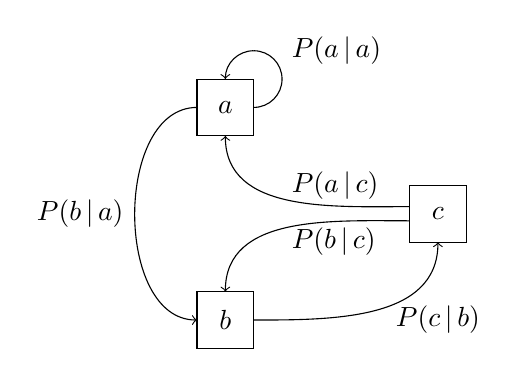
\begin{tikzpicture}[xscale=0.9,yscale=0.9]
%\draw[help lines] (-1,-0.5) grid (11,7.5);
%\draw (0,0) rectangle (10,8);
\draw (2,2) rectangle (2.8,2.8);
\draw (2.4,2.4) node[anchor=center] {$b$};
\draw (2,5) rectangle (2.8,5.8);
\draw (2.4,5.4) node[anchor=center] {$a$};
\draw (5,3.5) rectangle (5.8,4.3);
\draw (5.4,3.9) node[anchor=center] {$c$};
\draw [->] (2.8,2.4) to [out=0,in=-90] (5.4,3.5);
\draw [->] (5,3.8) to [out=180,in=90] (2.4,2.8);
\draw [->] (5,4) to [out=180,in=-90] (2.4,5);
\draw [->] (2,5.4) to [out=180,in=180] (2,2.4);
\draw (2.8,5.4) to [out=0,in=-90] (3.2,5.8);
\draw (3.2,5.8) to [out=90,in=0] (2.8,6.2);
\draw [->] (2.8,6.2) to [out=180,in=90] (2.4,5.8);
\draw (3.2,6.2) node[anchor=west] {$P(a\,\vert\,a)$};
\draw (1.1,3.9) node[anchor=east] {$P(b\,\vert\,a)$};
\draw (5.4,2.4) node {$P(c\,\vert\,b)$};
\draw (3.2,4.3) node[anchor=west] {$P(a\,\vert\,c)$};
\draw (3.2,3.5) node[anchor=west] {$P(b\,\vert\,c)$};
\end{tikzpicture}
\caption{Example transition graph for a discrete-time homogeneous Markov chain with a ternary state-space $\states=\{a,b,c\}$. The transition graph is a directed graph, with a vertex for each state, and an arc from the vertex of $x$ to that of $y$, with $x,y\in\states$, whenever $T(x,y)=P(X_1=y\,\vert\,X_0=x)>0$. The arcs are labelled with the corresponding transition probabilities. The figure uses the shorthand notation $P(y\vert x)$ for the elements $T(x,y)$ of $T$.}
\label{fig:example_trans_graph}
\end{figure}

One of the reasons transition graphs are sometimes useful, is that they allow one to study which parts of a system can be reached from other parts of the system. The simplest application is that of \emph{communicating states}:
\begin{definition}[Communicating States]\label{def:communicating_states}
Let $\{X_t\}_{t\in\natswith}$ be a discrete-time homogeneous Markov chain, and let $T$ be its associated transition matrix. For any two states $x,y\in\states$, $y$ is said to be \emph{accessible} from $x$ if there is some $n\in\nats$ such that $T^n(x,y)>0$. Furthermore, $x$ and $y$ are said to \emph{communicate} it $y$ is accessible from $x$, and $x$ is accessible from $y$. 
\end{definition}
Note that in the above, the term $T^n$ denotes the $n$-th matrix power of $T$ (c.f. Proposition~\ref{prop:markov_factor_transmat}). This has an intuitive graphical interpretation:
\begin{corollary}
Let $\{X_t\}_{t\in\natswith}$ be a discrete-time homogeneous Markov chain. Then for any $x,y\in\states$, $y$ is accessible from $x$ if and only if there is a path from $x$ to $y$ in the associated transition graph. Furthermore, $x$ and $y$ communicate if and only if there is a cycle in the associated transition graph that contains both $x$ and $y$.
\end{corollary}
\begin{proof}
Trivial from Definitions~\ref{def:trans_graph} and~\ref{def:communicating_states}.
\end{proof}
Inspection of the transition graph in Figure~\ref{fig:example_trans_graph} shows that, in that example, all states communicate with each other. When this is the case, i.e. when all states communicate, the Markov chain is said to be \emph{irreducible}. A maximal set of states that all communicate with each other is called a \emph{communication class}. Hence, an irreducible Markov chain has only a single communication class, which is equal to $\states$.

Note that not every Markov chain is irreducible; in general there may be more than one communication class. An example is given in Figure~\ref{fig:example_trans_graph_reducible}. When a communication class $\mathcal{A}\subset\states$ is accessible from a different communication class $\mathcal{B}\subset\states$, then $\mathcal{A}$ is said to dominate $\mathcal{B}$. A communication class which is not dominated is called \emph{maximal}. When a Markov chain has only a single maximal communication class, this is called the \emph{top (communication) class}. 
\begin{figure}
\centering
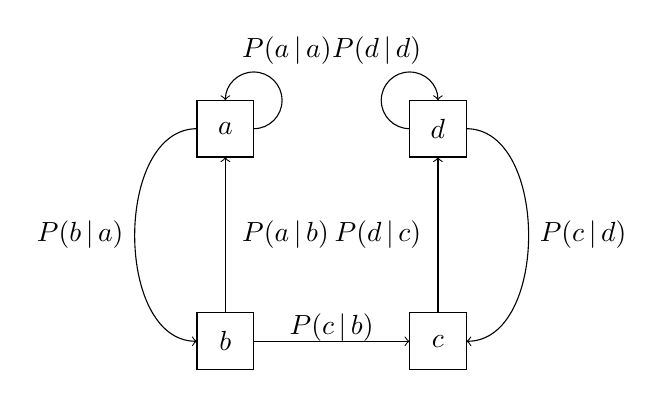
\begin{tikzpicture}[xscale=0.9,yscale=0.9]
%\draw[help lines] (-1,-0.5) grid (11,7.5);
%\draw (0,0) rectangle (10,8);
\draw (2,2) rectangle (2.8,2.8);
\draw (2.4,2.4) node[anchor=center] {$b$};
\draw (2,5) rectangle (2.8,5.8);
\draw (2.4,5.4) node[anchor=center] {$a$};
\draw (5,5) rectangle (5.8,5.8);
\draw (5.4,5.4) node[anchor=center] {$d$};
\draw (5,2) rectangle (5.8,2.8);
\draw (5.4,2.4) node[anchor=center] {$c$};
\draw [->] (2.8,2.4) to [out=0,in=180] (5,2.4);
\draw [->] (2.4,2.8) to [out=90,in=-90] (2.4,5);
\draw [->] (5.4,2.8) to [out=90,in=-90] (5.4,5);
%\draw [->] (5,3.8) to [out=180,in=90] (2.4,2.8);
%\draw [->] (5,4) to [out=180,in=-90] (2.4,5);
\draw [->] (2,5.4) to [out=180,in=180] (2,2.4);
\draw [->] (5.8,5.4) to [out=0,in=0] (5.8,2.4);
\draw (2.8,5.4) to [out=0,in=-90] (3.2,5.8);
\draw (3.2,5.8) to [out=90,in=0] (2.8,6.2);
\draw [->] (2.8,6.2) to [out=180,in=90] (2.4,5.8);
%
\draw (5,5.4) to [out=180,in=-90] (4.6,5.8);
\draw (4.6,5.8) to [out=90,in=180] (5,6.2);
\draw [->] (5,6.2) to [out=0,in=90] (5.4,5.8);
%
%\draw (5.4,2) to [out=-90,in=180] (5.8,1.6);
%\draw (5.8,1.6) to [out=0,in=-90] (6.2,2);
%\draw [->] (6.2,2) to [out=90,in=0] (5.8,2.4);
%
\draw (2.5,6.5) node[anchor=west] {$P(a\,\vert\,a)$};
\draw (1.1,3.9) node[anchor=east] {$P(b\,\vert\,a)$};
\draw (2.5,3.9) node[anchor=west] {$P(a\,\vert\,b)$};
\draw (5.3,6.5) node[anchor=east] {$P(d\,\vert\,d)$};
\draw (6.7,3.9) node[anchor=west] {$P(c\,\vert\,d)$};
\draw (5.3,3.9) node[anchor=east] {$P(d\,\vert\,c)$};
\draw (3.9,2.6) node[ ] {$P(c\,\vert\,b)$};
%\draw (5.4,2.4) node {$P(c\,\vert\,b)$};
%\draw (3.2,4.3) node[anchor=west] {$P(a\,\vert\,c)$};
%\draw (3.2,3.5) node[anchor=west] {$P(b\,\vert\,c)$};
\end{tikzpicture}
\caption{Transition graph of a Markov chain that is \emph{not} irreducible. It has two communication classes, $\{a,b\}$ and $\{c,d\}$. The set $\{c,d\}$ dominates $\{a,b\}$, and is the top (communication) class of the Markov chain. This Markov chain is top class regular.}
\label{fig:example_trans_graph_reducible}
\end{figure}

Investigation of the communicating states in a Markov chain is often useful when one is interested in the long-term behaviour of the system. After all, while a system might begin in one state, it need not necessarily always eventually return to that state; this is the property that is illustrated in Figure~\ref{fig:example_trans_graph_reducible}.

An important concept is that of the \emph{regularity} of the communication classes of a Markov chain. A communication class is regular if there is a number $n\in\nats$ such that it is possible to go from any state in the class, to any other state in the class, in exactly $n$ steps. Of particular importance is the notion of \emph{top class regularity}:
\begin{definition}[Top Class Regularity]
Let $\{X_t\}_{t\in\natswith}$ be a discrete-time homogeneous Markov chain, and let $T$ be its associated transition matrix. Then the Markov chain is said to be \emph{top class regular} if
\begin{equation*}
\bigl\{ y\in\states\,:\,(\exists n\in\nats)(\forall x\in\states)\, T^n(x,y)>0 \bigr\} \neq \emptyset\,,
\end{equation*}
and in that case the top class $\states_\mathrm{top}$ of the Markov chain exists and is equal to this set. When furthermore $\states_\mathrm{top}=\states$, the Markov chain itself is said to be \emph{regular}.
\end{definition}
The reason that this property is so important, is that it provides a sufficient condition for the long-term behaviour of a Markov chain to converge to a stationary distribution, regardless of the state in which it started:
\begin{theorem}
Let $\{X_t\}_{t\in\natswith}$ be a discrete-time homogeneous Markov chain, and let $T$ be its associated transition matrix. Let this Markov chain be regular. Then there exists a probability mass function $P_\infty:\states\to\realsnonneg$ such that, for all $x,y\in\states$, 
\begin{equation*}
P_\infty(y) = \lim_{n\to+\infty}T^n(x,y)\,.
\end{equation*}
\end{theorem}

\section{Imprecise Discrete-Time Markov Chains}\label{sec:idtmc}

%\emph{In this section: Parameterisation and imprecise local models. Different independence concepts. Different representations; sets of precise processes, (imprecise) event trees, imprecise graphical models. Computation using law of iterated lower expectation. Results on limit behaviour.}

%{\bf TODO: transition better into this section. }

We will now move on to the discussion surrounding \emph{Imprecise (Discrete-Time) Markov Chains} (IDTMCs). So, we still consider the time-dimension $\timedim=\natswith$. We will generalise each of the representations that we previously encountered to this new setting, where we roughly follow the same order as in Section~\ref{sec:prec_stoch_proc}. 

So, let us start with the ``measure-theoretic'' representation of imprecise stochastic processes. In this setting, we consider a \emph{set} $\mathbb{P}$ of probability measures on the measurable space of paths $(\Omega,\mathcal{F})$. Then for each $P\in\mathbb{P}$ we have a probability space $(\Omega,\mathcal{F},P)$, to which we can associate the precise stochastic process $\{X_t\}_{t\in\natswith}$ as in Definition~\ref{def:stochastic_process}. For any function $f\in\gambles(\states^n)$, $n\in\nats$, we can express the expected value on the $n$ time points $\mathbf{t}\subset\natswith$ as $\mathbb{E}_P[f(X_\mathbf{t})]$ as in Section~\ref{sec:prec_stoch_proc}. Recall from~\refIPChapter~that in this imprecise probabilistic context, we are more generally interested in the \emph{lower-} and \emph{upper expectation} of $f$, which are defined respectively as
\begin{equation*}
\underline{\mathbb{E}}_\mathbb{P}\bigl[f(X_\mathbf{t})\bigr] \coloneqq \inf_{P\in\mathbb{P}} \mathbb{E}_P\bigl[f(X_\mathbf{t})\bigr],\quad\text{and,}\quad \overline{\mathbb{E}}_\mathbb{P}\bigl[f(X_\mathbf{t})\bigr] \coloneqq \sup_{P\in\mathbb{P}} \mathbb{E}_P\bigl[f(X_\mathbf{t})\bigr]\,.
\end{equation*}
We briefly recall the well-known conjugacy relation $\overline{\mathbb{E}}_\mathbb{P}\bigl[f(X_\mathbf{t})\bigr]=-\underline{\mathbb{E}}_\mathbb{P}\bigl[-f(X_\mathbf{t})\bigr]$, from which it follows that we can present the remainder of this discussion entirely in terms of lower expectations; any results on upper expectations follow analogously through this relation.

Slightly more generally than the above, we will focus on \emph{conditional} lower expectations. Similar to the precise case that we discussed before, these are defined for any $f\in\gambles(\states^{n+m})$, $n,m\in\nats$, any $\mathbf{s},\mathbf{t}\subset\natswith$ such that $\mathbf{s}$ and $\mathbf{t}$ are of length $n$ and $m$ respectively, and any $x_\mathbf{s}\in\states^n$, as
\begin{equation*}
\underline{\mathbb{E}}_\mathbb{P}\bigl[f(X_\mathbf{s},X_\mathbf{t})\,\big\vert\,X_\mathbf{s}=x_\mathbf{s}\bigr] \coloneqq \inf_{P\in\mathbb{P}} \mathbb{E}_P \bigl[f(X_\mathbf{s},X_\mathbf{t})\,\big\vert\,X_\mathbf{s}=x_\mathbf{s}\bigr]\,,
\end{equation*}
whenever $\underline{\mathbb{E}}_\mathbb{P}[\mathbb{I}_{x_\mathbf{s}}(X_\mathbf{s})]>0$. In this last condition, $\mathbb{I}_{x_\mathbf{s}}(\cdot)$ is the indicator of $x_\mathbf{s}$; for all $y_\mathbf{s}\in\states^n$, $\mathbb{I}_{x_\mathbf{s}}(y_\mathbf{s})\coloneqq 1$ if $x_\mathbf{s}=y_\mathbf{s}$, and $\mathbb{I}_{x_\mathbf{s}}(y_\mathbf{s})\coloneqq 0$, otherwise. Note that then
\begin{equation*}
0 < \underline{\mathbb{E}}_\mathbb{P}[\mathbb{I}_{x_\mathbf{s}}(X_\mathbf{s})] = \inf_{P\in\mathbb{P}} \mathbb{E}_P[\mathbb{I}_{x_\mathbf{s}}(X_\mathbf{s})] = \inf_{P\in\mathbb{P}} P(X_\mathbf{s}=x_\mathbf{s})\,,
\end{equation*}
so this condition guarantees that the conditional expectations are well-defined for all the precise measures $P\in\mathbb{P}$.

We are now ready to give the formal definition of an imprecise discrete-time Markov chain (IDTMC):
\begin{definition}[IDTMC as Set of Processes]\label{def:idtmc_set_measures}
An \emph{imprecise discrete-time Markov chain} is a set $\mathbb{P}$ of probability measures on the measurable space $(\Omega,\mathcal{F})$, with associated lower expectation operator $\underline{\mathbb{E}}_\mathbb{P}$ as defined above, such that, for all $f\in\gambles(\states)$ and all $s_1,\ldots,s_n,t\in\natswith$ such that $s_1<\cdots s_n<t$,
\begin{equation*}
\underline{\mathbb{E}}_\mathbb{P}\bigl[f(X_t)\,\big\vert\, X_{s_1},\ldots,X_{s_n}\bigr] = \underline{\mathbb{E}}_\mathbb{P}\bigl[f(X_t)\,\big\vert\, X_{s_n}\bigr]\,.
\end{equation*}
Furthermore, an imprecise discrete-time Markov chain is called \emph{homogeneous} if, for all $s,t\in\natswith$, $s<t$, and all $f\in\gamblesX$, it holds that $\underline{\mathbb{E}}_\mathbb{P}[f(X_t)\,\vert\,X_s]= \underline{\mathbb{E}}_\mathbb{P}[f(X_{t-s})\,\vert\,X_0]$.
\end{definition}
Let us compare this with Definition~\ref{def:measure_markov}, the measure-theoretic definition of a precise Markov chain. The first difference is that the imprecise definition above is phrased in terms of (lower) expectations, whereas the precise definition used probabilities. We recall that this is because, in the framework of imprecise probability, it does not suffice to state results in terms of (lower) probabilities; instead the more general language of (lower) expectation operators is required. %{\bf *** TODO: this needs some polish depending on how Chapter 2 discussed this}

Nevertheless, this definition implies that, in terms of lower probabilities,
\begin{align*}
\inf_{P\in\mathbb{P}} P(X_t=x\,\vert\,X_{s_1},\ldots,X_{s_n}) &= 
\underline{\mathbb{E}}_\mathbb{P}\bigl[\mathbb{I}_{x}(X_t)\,\big\vert\, X_{s_1},\ldots,X_{s_n}\bigr] \\
 &= \underline{\mathbb{E}}_\mathbb{P}\bigl[\mathbb{I}_{x}(X_t)\,\big\vert\, X_{s_n}\bigr]
= \inf_{P\in\mathbb{P}} P(X_t=x\,\vert\,X_{s_n})\,,
\end{align*}
which displays this imprecise Markov condition in more familiar terms.

One may wonder at this point whether an imprecise Markov chain $\mathbb{P}$ is itself a set of Markov chains; the answer to this question is a resounding \emph{no} (or at least, not necessarily). This point deserves the strongest possible emphasis:
\quad\newline\newline
\noindent \emph{An element of an imprecise Markov chain $\mathbb{P}$ does {\bf not} need to be a Markov chain! So, in general $P(X_t\,\vert\,X_{s_1},\ldots,X_{s_n})\neq P(X_t\,\vert\,X_{s_n})$ for $P\in\mathbb{P}$, with $s_1<\cdots s_n<t$ in $\natswith$.}
\quad\newline\newline
To clarify, the ``imprecise Markov condition'' of an imprecise Markov chain is an ``independence'' assessment about the \emph{lower envelope} only. Formally, it is an assessment of \emph{epistemic irrelevance}---a specific type of independence that arises in imprecise probability theory---which is weaker than \emph{strong independence}---a different type of independence, and what would hold of all $P\in\mathbb{P}$ were Markov chains.

In a similar vein, the notion of homogeneity is here only enforced on the lower envelope. So, for an IDTMC $\mathbb{P}$ that is homogeneous, there may be processes $P\in\mathbb{P}$ that are neither Markov, nor homogeneous.

The reason that we stress this so much is twofold. First of all, it implies that the structural assumptions of an imprecise Markov chain are in fact much weaker than those of a precise Markov chain---we no longer assume that future events are fully independent of the history, given the current state, or that their distribution is independent of the point in time. They might be, of course---there \emph{are} elements $P\in\mathbb{P}$ that satisfy those properties---but it's not enforced as strictly. In other words, this model also represents ``higher-order'' uncertainty about the \emph{structural properties} of the system that we are trying to model.

The second reason is that this property is central to all the efficient computational methods that have been developed for working with imprecise Markov chains. We will next illustrate this point by moving the discussion to the representation of IDTMCs as \emph{imprecise probability trees}.

%{\bf TODO: blabla, alleen op de envelop (epistemic irrelevance, zie chapter 2?), daardoor (veel) zwakkere aanname. Wel cruciaal voor computationele technieken! Verder, ook analoog voor impreciese homogeniteit.}
\subsection{Imprecise Probability Trees}\label{sec:imprecise_prob_tree}
Recall that for precise probability trees, we associate with each situation $w\in\states^*_\Box$ a local model $p_w$, which is a probability mass function on $\states$. In contrast, in order to define \emph{imprecise} probability trees, we will consider \emph{imprecise local models}. Such an imprecise local model $\mathcal{P}_w$ is simply a \emph{set} of probability mass functions on $\states$. This leads to the following definition:
\begin{definition}[Imprecise Probability Tree]
An imprecise probability tree is a tuple $(\states^*_\Box,\prec,\mathcal{P}_{(\cdot)})$, where $(\states^*_\Box,\prec)$ is an event tree, and $\mathcal{P}_{(\cdot)}$ is a set-valued function such that, for all $w\in\states^*_\Box$, $\mathcal{P}_w$ is a non-empty set of probability mass functions on $\states$.
\end{definition}
An obvious question is how one should interpret such imprecise probability trees. As a first step, we consider the (precise) probability trees that are \emph{compatible} with a given imprecise probability tree:
\begin{definition}
Let $(\states^*_\Box,\prec,\mathcal{P}_{(\cdot)})$ be an imprecise probability tree. Then a (precise) probability tree $(\states^*_\Box,\prec,p_{(\cdot)})$ is called \emph{compatible} with this imprecise probability tree, if $p_w\in\mathcal{P}_w$ for all $w\in \states^*_\Box$.
\end{definition}

This immediately lets us connect back to the sets-of-measures that we discussed before. Specifically, consider an imprecise probability tree $(\states^*_\Box,\prec,\mathcal{P}_{(\cdot)})$, and suppose the tree $(\states^*_\Box,\prec,p_{(\cdot)})$ is compatible with it. Then, using the method outlined in Section~\ref{sec:prob_trees}, we can associate a (precise) measure $P$ to this precise tree. Collecting in the set $\mathbb{P}$ all the associated measures of all precise trees that are compatible with the imprecise tree, we obtain the set-representation from Section~\ref{sec:idtmc}. The connection in the other direction is analogous.

With this connection in place, we can again start to consider computational methods for lower expectations. Analogous to what we have seen before, in this context we have a \emph{law of iterated lower expectation} that we can use as a computational tool. The imprecise probability tree representation again provides graphical intuition.

Similar to the exposition in Section~\ref{sec:prob_trees}, we start with a function $f\in\gambles(\states^{n+1})$ of which we want to compute the lower expectation with respect to the states at the time points $0,\ldots,n$. Then for any situation $w\in\states^*$ such that $\lvert w\rvert = n+1$, the lower expectation is trivial:
\begin{equation*}
\underline{\mathbb{E}}_\mathbb{P}\left[f(X_{0:n})\,\big\vert\,X_{0:n}=w\right] = f(w)\,.
\end{equation*}
We then again ``pull back'' to the parent situation $v$ of $w$; this is where the main difference with Section~\ref{sec:prob_trees} occurs. Notably, we here have an \emph{imprecise} local model $\mathcal{P}_v$ associated to this node $v$. The point to the law of iterated lower expectation, is that it suffices to only compute the associated conditional lower expectation locally:
\begin{equation*}
\underline{\mathbb{E}}_\mathbb{P}\left[f(X_{0:n})\,\big\vert\,X_{0:(n-1)}=v\right] = \inf_{p_v\in\mathcal{P}_v} \sum_{x\in\states} p_v(x) \underline{\mathbb{E}}_\mathbb{P}\left[f(X_{0:n})\,\big\vert\,X_{0:(n-1)}=v,X_n=x\right]\,.
\end{equation*}
Exactly analogous to the precise case, by repeatedly pulling back until we reach the root of the tree we eventually compute
\begin{equation*}
\underline{\mathbb{E}}_\mathbb{P}\left[ f(X_{0:n})\right] = \inf_{p_\Box\in\mathcal{P}_\Box} \sum_{x\in\states} p_\Box(x) \underline{\mathbb{E}}_\mathbb{P}\left[ f(X_{0:n})\,\big\vert\,X_0=x\right]\,,
\end{equation*}
which is the lower expectation of interest.

As before, the need to specify these (imprecise) local models $\mathcal{P}_w$ for all situations $w\in\states^*_\Box$ makes such a model difficult to work with. This is simplified for imprecise Markov chains; note that we here assume the analogue of homogeneity to hold implicitly:
\begin{definition}[Homogeneous IDTMC as Imprecise Probability Tree]\label{def:idtmc_prob_tree}
An imprecise probability tree $(\states^*_\Box,\prec,\mathcal{P}_{(\cdot)})$ is called an imprecise homogeneous discrete-time Markov chain if, for all $v,w\in\states^*$ for which $v_\top=w_\top$, it holds that $\mathcal{P}_v=\mathcal{P}_w$.
\end{definition}
\begin{corollary}
Let $(\states^*_\Box,\prec,\mathcal{P}_{(\cdot)})$ be a homogeneous IDTMC. Then for all $x\in\states$ and all $w\in\states^*$ such that $w_\top=x$, it holds that $\mathcal{P}_w=\mathcal{P}_x$.
\end{corollary}
\begin{proof}
Trivial from Definition~\ref{def:idtmc_prob_tree} and the fact that all $x\in\states$ are also situations.
\end{proof}
As above, an IDTMC $(\states^*_\Box,\prec,\mathcal{P}_{(\cdot)})$ has a set of compatible precise probability trees, each of which induces a measure $P$, and these are collected in the set $\mathbb{P}$, which is the measure-theoretic IDTMC representation from Definition~\ref{def:idtmc_set_measures}. Observe that a precise probability tree does \emph{not} have to be a (homogeneous) Markov chain, for it to be compatible with a given IDTMC! That is, to be compatible each local model $p_w$, $w\in\states^*_\Box$, should be in the set $\mathcal{P}_{w_\top}$, and this set only depends on the most recent state $w_\top$ of the situation $w$. But, while in a different situation $v$ such that $v_\top=w_\top$, we do require that $p_v\in\mathcal{P}_{v_\top}=\mathcal{P}_{w_\top}$, we do \emph{not} require that $p_v=p_w$!

We will next illustrate that the law of iterated lower expectation simplifies further for imprecise Markov chains. We do this again by considering the imprecise analogue of probabilistic graphical models.

\subsection{Credal Networks}\label{sec:credal_net}

We here consider the graphical representation of imprecise Markov chains as \emph{credal networks}. This is the imprecise generalisation of the PGM representation that we encountered in Section~\ref{sec:pgm}. The graphical structure is as before, with the notable differences being (i) the local models (which are here replaced with imprecise local models), and (ii) the interpretation of the independence properties induced by the arcs. Regarding the second point, it suffices for our present purpose to note that we interpret the structure as a credal network under epistemic irrelevance. This then has the same consequence as that stated in the beginning of Section~\ref{sec:idtmc}: given the value of the parent of a node $X_t$, $t\in\natswith$, the lower expectation of any function dependent on $X_t$ does not depend on the values of the non-parents, non-descendants (again, grandparents and so on) of $X_t$. For reference, the graphical representation is drawn in Figure~\ref{fig:example_markov_credal}.

\begin{figure}
\centering
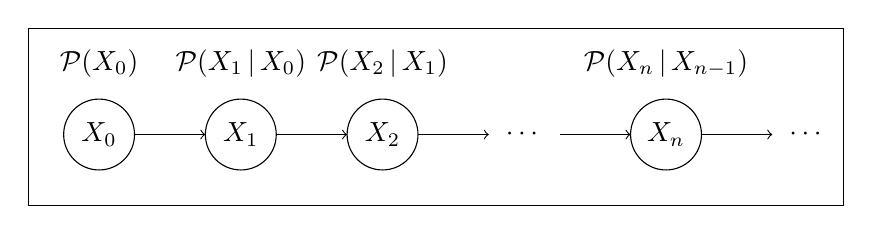
\begin{tikzpicture}[xscale=0.9,yscale=0.9]
%\draw[help lines] (-1,-0.5) grid (11,7.5);
\draw (-1,-1) rectangle (10.5,1.5);
\draw (0,0) circle(0.5) node[align=center] {$X_0$};
\draw (0,1) node[align=right] {$\mathcal{P}(X_0)$};
\draw [->] (0.5,0) -- (1.5,0);
\draw (2,0) circle(0.5) node[align=center] {$X_1$};
\draw (2,1) node[align=right] {$\mathcal{P}(X_1\,\vert\,X_0)$};
\draw [->] (2.5,0) -- (3.5,0);
\draw (4,0) circle(0.5) node[align=center] {$X_2$};
\draw (4,1) node[align=right] {$\mathcal{P}(X_2\,\vert\,X_1)$};
\draw [->] (4.5,0) -- (5.5,0);
\draw (6,0) node[align=right] {$\cdots$};
\draw [->] (6.5,0) -- (7.5,0);
\draw (8,0) circle(0.5) node[align=center] {$X_n$};
\draw (8,1) node[align=right] {$\mathcal{P}(X_n\,\vert\,X_{n-1})$};
\draw [->] (8.5,0) -- (9.5,0);
\draw (10,0) node[align=right] {$\cdots$};
\end{tikzpicture}
\caption{Credal network representation of an imprecise discrete-time Markov chain. An incoming arc on a node represents that the local uncertainty model of the corresponding variable is influenced by the originating node of that arc. Correspondingly, each node associates an imprecise probability model to its variable, conditional on the values of the random variables of the nodes on which it is dependent.}
\label{fig:example_markov_credal}
\end{figure}
The interpretation in terms of sets of distributions is as would be expected; the model induces a set $\mathbb{P}$, each $P\in\mathbb{P}$ of which satisfies $P(X_n\,\vert\,X_{n-1})\in\mathcal{P}(X_n\,\vert\,X_{n-1})$ for all $n\in\nats$, and $P(X_0)\in\mathcal{P}(X_0)$. As before, the independence assumptions are not necessarily required to hold for these compatible precise models. Conversely, if we are given an IDTMC $\mathbb{P}$, then the local models $\mathcal{P}(X_n\vert X_{n-1})$ of the credal network are constructed by restricting attention to the conditional events $P(X_{n}\,\vert\,X_{n-1})$, and varying $P$ over $\mathbb{P}$. So, we can straightforwardly switch between representations.

We next generalise the exposition in Section~\ref{sec:pgm} regarding the associated transition matrices. To this end, fix any $t\in\natswith$. Then, as in the precise case, each element $P(X_{t+1}\,\vert\,X_t)\in\mathcal{P}(X_{t+1}\,\vert\,X_t)$ induces a transition matrix $T_t$. So, let us now consider the \emph{set} $\mathcal{T}_t$ of transition matrices that is induced by the imprecise local models:
\begin{align*}
\mathcal{T}_t \coloneqq \Bigl\{ T_t\,&:\, \bigl(\forall x,y\in\states\,:\, T_t(x,y)=P(X_{t+1}=y\,\vert\,X_t=x)\bigr), \\
 &\quad P(X_{t+1}\,\vert\,X_t)\in\mathcal{P}(X_{t+1}\,\vert\,X_t) \Bigr\}\,.
\end{align*} 
A key insight is that we can use this set of transition matrices to define a convenient computational tool for lower expectations:
\begin{definition}\label{def:lower_discrete_trans}
Let $\mathbb{P}$ be an IDTMC, and let $\mathcal{T}_t$ be the associated family of sets of transition matrices, as defined above. Then, for each $t\in\natswith$, the associated \emph{lower transition operator} $\underline{T}_t:\gamblesX\to\gamblesX$ is defined, for all $f\in\gamblesX$ and all $x\in\states$, as
\begin{equation*}
\bigl[\underline{T}_tf\bigr](x) \coloneqq \inf_{T_t\in\mathcal{T}_t}\bigl[T_tf\bigr](x)\,.
\end{equation*}
\end{definition}
This lower transition operator essentially fulfils the same role as the transition matrices from which it is derived. In particular, we have the following:
\begin{proposition}\label{prop:lower_trans_is_lower_exp}
Let $\mathbb{P}$ be an IDTMC, and let $\underline{T}_t$ be the associated family of lower transition operators. Then, for all $t\in\natswith$ and all $f\in\gamblesX$, it holds that
\begin{equation*}
\underline{T}_tf = \underline{\mathbb{E}}_\mathbb{P}\bigl[f(X_{t+1})\,\vert\,X_t\bigr]\,.
\end{equation*}
\end{proposition}
\begin{proof}
Simply use the definitions together with Proposition~\ref{prop:expectation_using_transmat}. For any $x\in\states$,
\begin{align*}
\bigl[\underline{T}_tf\bigr](x) = \inf_{T_t\in\mathcal{T}_t} \bigl[T_tf\bigr](x) &= \inf_{T_t\in\mathcal{T}_t} \sum_{y\in\states} f(y) T_t(x,y) \\
 &= \inf_{P(X_{t+1}\vert X_t)\in\mathcal{P}(X_{t+1}\vert X_t)} \sum_{y\in\states} f(y) P(X_{t+1}=y\vert X_t=x) \\
 &= \inf_{P\in\mathbb{P}} \sum_{y\in\states} f(y) P(X_{t+1}=y\vert X_t=x) \\
 &= \inf_{P\in\mathbb{P}} \mathbb{E}_P\bigl[f(X_{t+1})\,\big\vert\,X_t=x\bigr] = \underline{\mathbb{E}}_\mathbb{P}\bigl[f(X_{t+1})\,\big\vert\,X_t=x\bigr]\,,
\end{align*}
where in the fourth equality we used the definition of the compatible measures.
\end{proof}
As in Corollary~\ref{cor:trans_mat_loie}, we can now state the simplified law of iterated lower expectation for imprecise Markov chains, using these lower transition operators:
\begin{theorem}\label{thm:loile_dt}
Let $\mathbb{P}$ be an IDTMC, and let $\underline{T}_t$ be the associated family of lower transition operators. Then, for all $f\in\gamblesX$, all $s,t\in\natswith$ such that $s\leq t$, and all $x\in\states$, it holds that
\begin{equation*}
\underline{\mathbb{E}}_\mathbb{P}\bigl[f(X_t)\,\big\vert\,X_s=x\bigr] = \bigl[\underline{T}_s\cdots \underline{T}_tf\bigr](x)\,,
\end{equation*}
where the right-hand side represents an iterated operator product (composition). 
\end{theorem}
We omit the full proof, but the interested reader can reconstruct the argument by using the general computational process of iterated lower expectation as explained in Section~\ref{sec:imprecise_prob_tree}, the imprecise Markov property from Definition~\ref{def:idtmc_set_measures}, and the interpretation of the lower transition operator from Proposition~\ref{prop:lower_trans_is_lower_exp}.

\subsection{Limits of Homogeneous IDTMCs}

We conclude the discussion of imprecise discrete-time Markov chains with some results about their limit behaviour, in analogy to the results in Section~\ref{sec:trans_graph}. We start again by restricting attention to homogeneous IDTMCs, and notice the following (we omit the proof, which is straightforward):
\begin{proposition}
Let $\mathbb{P}$ be a homogeneous IDTMC, and let $\underline{T}_t$ be the associated family of lower transition operators. Then there is a unique lower transition operator $\underline{T}:\gamblesX\to\gamblesX$, such that, for all $f\in\gamblesX$, $\underline{T}_tf=\underline{T}f$ for all $t\in\natswith$.
\end{proposition}

We take a moment here to remark on a property that was already encountered in~\refIPChapter: the duality between lower expectation operators and closed and convex sets of probability measures. Indeed, this correspondence was also used in Definition~\ref{def:lower_discrete_trans} above, where we used the sets $\mathcal{T}_t$ of transition matrices, to construct the lower transition operator $\underline{T}_t$. Since, as we have just seen, the dynamics of a \emph{homogeneous} IDTMC can be completely described by a single $\underline{T}$, it now makes sense to think about the other direction. 

Specifically, corresponding to $\underline{T}$ there exists a closed and convex set $\mathcal{T}$ of transition matrices, such that $\underline{T}f=\inf_{T\in\mathcal{T}}Tf$ for all $f\in\gamblesX$. This implies that (up to the initial distribution at time zero) an IDTMC can also be characterised by such a set $\mathcal{T}$. So, whereas we noted in Section~\ref{sec:pgm} that a (precise) discrete-time Markov chain's canonical parameter is a single transition matrix $T$, for a homogeneous IDTMC the parameter can be understood as a single closed and convex set $\mathcal{T}$ of transition matrices.

Furthermore, in Section~\ref{sec:pgm} we used a property of the associated transition matrix $T$, to state a sufficient condition for the long-term behaviour of the Markov chain to converge to a distribution over the states, independently of the state in which it started. We here have a similar result, which starts by introducing the conjugate \emph{upper} transition operator $\overline{T}:\gamblesX\to\gamblesX:f\mapsto -\underline{T}(-f)$.

Now, recall that in the precise case, a homogeneous discrete-time Markov chain with transition matrix $T$ was said to be \emph{regular}, if there was some $n\in\nats$ such that $T^n(x,y)>0$ for all $x,y\in\states$. The interpretation is clear: the Markov chain is regular if and only if there is some finite number of steps $n$ in which every state $x$ can reach every state $y$. This is now generalised to the imprecise case:
\begin{definition}[Regularity for Homogeneous IDTMC]
Let $\mathbb{P}$ be a homogeneous IDTMC with associated lower (and upper) transition operator $\underline{T}$ (and $\overline{T}$). Then the IDTMC is \emph{regular} if there is some $n\in\nats$ such that $\bigl[\overline{T}^n\mathbb{I}_y\bigr](x)>0$ for all $x,y\in\states$.
\end{definition}
Let us consider this definition. One difference with the precise case, is the introduction of the indicator function $\mathbb{I}_y$ on the state $y\in\states$; this was introduced because, in contrast to matrices, we cannot index the ``elements'' of the transition operator. Specifically, using Theorem~\ref{thm:loile_dt}, we can interpret the condition as
\begin{equation*}
0 < \Bigl[\overline{T}^n\mathbb{I}_y\Bigr](x) = \overline{\mathbb{E}}_\mathbb{P}\bigl[\mathbb{I}_y(X_n)\,\big\vert\,X_0=x\bigr] = \sup_{P\in\mathbb{P}} P(X_n=y\,\vert\,X_0=x)\,,
\end{equation*}
for all $x,y\in\states$ and some $n\in\nats$. What regularity asks for, then, is for there to be some $n\in\nats$ such that is possible for all $x,y\in\states$ to move from $x$ to $y$ in exactly $n$ steps, \emph{according to some} $P\in\mathbb{P}$. In particular, the (precise) measure $P$ for which this needs to be possible, can be different for every pair $x,y\in\states$. Regularity for IDTMCs then, is a much weaker---easier to satisfy---condition than that for precise Markov chains. Nevertheless, the condition is sufficient for the following:

\begin{theorem}\label{theo:idtmc_ergodic_simple}
Let $\mathbb{P}$ be a homogeneous IDTMC with associated lower transition operator $\underline{T}$, and suppose that $\mathbb{P}$ is regular. Then, there exists a unique lower expectation operator $\underline{\mathbb{E}}_\mathbb{P}[\cdot(X_{+\infty})]:\gamblesX\to\reals$ such that, for all $f\in\gamblesX$ and all $x\in\states$,
\begin{equation*}
\underline{\mathbb{E}}_\mathbb{P}\bigl[f(X_{+\infty})\bigr] = \lim_{n\to+\infty} \underline{\mathbb{E}}_\mathbb{P}\bigl[f(X_n)\,\vert\,X_0=x\bigr] = \lim_{n\to+\infty} \bigl[\underline{T}^nf\bigr](x)\,.
\end{equation*}
Furthermore, this is the unique $\underline{T}$-invariant lower expectation on $\gamblesX$, meaning that $\underline{\mathbb{E}}_\mathbb{P}[f(X_{+\infty})]= \underline{\mathbb{E}}_\mathbb{P}\bigl[[\underline{T}\,f](X_{+\infty})\bigr]$ for all $f\in\gamblesX$.
\end{theorem}

\section{Imprecise Continuous-Time Markov Chains}\label{sec:ictmc}

%\emph{In this section: Intuition as limit of discrete-time (imprecise) Markov chains. Parametrisation using local models and the (imprecise) matrix exponential. Recollection and translation of the different independence concepts. Different representations; sets of precise processes and imprecise graphical models. Reduction of computations to discrete-time case, and law of iterated lower expectation. Results on limit behaviour.}

We now move on to the discussion about (imprecise) \emph{continuous}-time Markov chains. We have already encountered this setting several times in the preceding discussions, but have generally skipped over any details. Let us recall from Section~\ref{sec:prec_stoch_proc} that continuous-time stochastic processes are identified with a time-dimension $\timedim=\realsnonneg$, and that the elements $\omega$ of the outcome space of paths $\Omega$ are maps $\omega:
\realsnonneg\to\states$. The measure-theoretic definition is then as before, where we consider the abstract probability space $(\Omega,\mathcal{F},P)$, and the stochastic process $\{X_t\}_{t\in\realsnonneg}$ is a family of random variables on this space. Furthermore, measure-theoretic definitions of (homogeneous) continuous-time Markov chains (CTMCs) were already encountered in Definitions~\ref{def:measure_markov} and~\ref{def:measure_homogen_markov}.

How, then, can these models be interpreted? Let us start by considering the simplest case, \emph{viz.}, a precise and homogeneous Markov chain in continuous-time. According to the previous definitions, this is a stochastic process such that
\begin{enumerate}
\item $P(X_t\,\vert\, X_{s_1},\ldots,X_{s_n}) = P(X_t\,\vert\,X_{s_n})$ for all $s_1<\cdots<s_n<t$ in $\realsnonneg$, and 
\item $P(X_t\,\vert\,X_s) = P(X_{t-s}\,\vert\,X_0)$ for all $s<t$ in $\realsnonneg$.
\end{enumerate}
The immediate difficulty of moving on from this abstract representation is that the time-dimension is now, in a sense, too big to use any of the previous representations. For instance, we could try to draw a ``continuous-time'' probability tree, where the local model of a situation with terminal state $w_\top$ is given by a probability mass function $P(X_{t}\,\vert\,X_0=w_\top)$. But what is the time $t$ that we should use? When we were working in discrete-time, the approach was to use the \emph{next} time point, as viewed from the current situation. But of course, there is no ``next'' time $t$ when working in continuous-time! This difficulty of using graphical representations is the main reason that we have postponed the treatment of continuous-time processes until now, thereby hopefully allowing the reader to first develop some graphical intuition for the discrete-time case.

Nevertheless, all is not lost; the first interpretation that we will consider is to view continuous-time processes as limits of discrete-time ones. To this end, it will be convenient to consider the transition-matrix $T$ associated with a homogeneous DTMC. Let us recall from Sections~\ref{sec:pgm} and~\ref{sec:trans_graph}, that the elements of such a matrix represent the ``transition probabilities'' of the system, that is, the probability of moving from a state $x$ to a state $y$, in one time step:
\begin{equation*}
T(x,y) = P(X_1=y\,\vert\,X_0=x)\,.
\end{equation*}
We can use this formalism to interpret the continuous-time case, by simply ``fixing the length of the step''. That is, consider some ``step size'' $\Delta>0$. Then, for a homogeneous CTMC, we known that
\begin{equation*}
P(X_{t+\Delta}\,\vert\,X_t) = P(X_\Delta\,\vert\,X_0)\,,
\end{equation*}
for all $t\in\realsnonneg$, so we can collect these ``transition probabilities'' in a matrix $T_\Delta$:
\begin{equation*}
T_\Delta(x,y) \coloneqq P(X_\Delta=y\,\vert\,X_0=x)\quad\quad\text{for all }x,y\in\states\,.
\end{equation*}
Clearly, the elements of $T_\Delta$ are the probabilities for the system to end up in a state $y$, if it is currently in a state $x$, after a time duration of $\Delta$ has elapsed. Provided, then, that we are not interested in a granularity of the time dimension that is finer than $\Delta$, this representation suffices. The matrix $T_\Delta$ can be associated with a DTMC, and all the previous results can be used. For instance, for any multiple $n\in\nats$ of $\Delta$, we use Proposition~\ref{prop:markov_factor_transmat} to find that
\begin{equation*}
P(X_{n\Delta}=y\,\vert\,X_0=x) = T_\Delta^n(x,y)\,.
\end{equation*}

But, of course, the point of using the continuous-time representation is that we \emph{are} interested in an arbitrarily fine granularity of the time-dimension. In particular, the measure-theoretic definition encodes this arbitrary granularity, and it seems a waste to only focus on the restriction to a single step size $\Delta$. The ``trick'', then, is to take the limit as $\Delta$ goes to zero, and somehow usefully represent this limit. It is hopefully clear from the above discussion that, as we decrease $\Delta$ further and further, the associated transition matrix $T_\Delta$ covers increasingly smaller steps along the time-dimension. And, for each such positive $\Delta$, we can associate a discrete-time Markov chain, and use all the previous interpretations that we developed.

We first remark that the naive limit does not encode a lot of information; ignoring possible issues of continuity, it trivially holds that
\begin{equation}\label{eq:time_zero_is_id}
\lim_{\Delta\to 0^+} P(X_{\Delta}=y\,\vert\,X_0=x) = P(X_0=y\,\vert\,X_0=x) = \begin{cases}
1 & \text{if $y=x$, and} \\
0 & \text{otherwise.}
\end{cases}
\end{equation}
In matrix notation this reads as $\lim_{\Delta\to0^+}T_\Delta = I$, where $I$ denotes the $\lvert\states\rvert\times \lvert\states\rvert$ identity matrix. Colloquially, we might understand this as saying that ``if time does not evolve, the system does not change''. This is clearly an almost tautological statement to make of what should be interpreted as a dynamical system. So let us consider how the system \emph{does} change as time evolves. The natural representation for this is obviously the \emph{derivative} of the transition matrix $T_\Delta$; this is the limit interpretation that we shall use. Ignoring technical issues of differentiability, we have
\begin{equation}\label{eq:rate_mat_is_deriv}
\frac{\mathrm{d}\,T_\Delta}{\mathrm{d}\,\Delta}\bigg\vert_{\Delta=0} = \lim_{\Delta\to0^+}\frac{T_\Delta - I}{\Delta} =: Q\,,
\end{equation}
where we have used the previous observation that $T_0=I$. On the right-hand side, the term $Q$ is called the \emph{transition rate matrix} of the homogeneous CTMC (or sometimes simply the \emph{rate matrix}). It is clear from the above definition that it encodes the \emph{rate of change} of the transition probabilities around time zero. It satisfies the following properties:
\begin{definition}[Transition Rate Matrix]\label{def:trans_rate_matrix}
A real-valued $\lvert\states\rvert\times\lvert\states\rvert$ matrix $Q$ is called a \emph{transition rate matrix} if, for all $x\in\states$, it holds that
\begin{enumerate}
\item $Q(x,y)\geq 0$ for all $y\in\states$ such that $x\neq y$, and
\item $\sum_{y\in\states}Q(x,y)=0$.
\end{enumerate}
\end{definition}
The elements $Q(x,y)$ of a rate matrix can be interpreted as the ``speed'' with which the process moves from the state $x$ to the state $y$. In the above definition, the two conditions imply that the diagonal elements $Q(x,x)$ are always non-positive. On the other hand, the first condition states that the off-diagonal elements are non-negative. Combined this can be understood as saying that the system will move ``out'' of the current state (the non-positivity of the diagonal elements) and ``into'' some other states (the non-negativity of the off-diagonals).

A more concrete way to interpret the rate-matrix, is through a linearised approximation of the transition probabilities over a small enough time-step. That is, it follows from Equation~\eqref{eq:rate_mat_is_deriv} that, for ``small enough'' $\Delta>0$, it holds that $Q\approx (T_\Delta-I)\nicefrac{1}{\Delta}$; hence also
\begin{equation}\label{eq:cont_trans_small_delta}
T_\Delta \approx I + \Delta Q\,.
\end{equation}
We therefore see that the matrix $Q$ can be used to approximately compute the transition probabilities over a small enough time step.

An obvious next question is if we can extrapolate this to compute the matrix $T_t$ that contains the transition probabilities over an arbitrary duration $t$. Indeed we can, although it requires a bit of setup. For any $t\in\realsnonneg$, first define the transition matrix of the CTMC after time $t$:
\begin{equation*}
T_t(x,y) \coloneqq P(X_{t}=y\,\vert\,X_0=x)\quad\quad\text{for all }x,y\in\states\,.
\end{equation*}
Then we differentiate in $t$; to this end, first fix $\Delta>0$, and use the Markov property and homogeneity to derive that $T_{t+\Delta} = T_tT_\Delta=T_\Delta T_t$ (c.f. Proposition~\ref{prop:markov_factor_transmat}). Then we proceed by using Equation~\eqref{eq:rate_mat_is_deriv}:
\begin{equation*}
\frac{\mathrm{d}\,T_t}{\mathrm{d}\,t} = \lim_{\Delta\to0^+} \frac{T_{t+\Delta} - T_t}{\Delta} = \lim_{\Delta\to0^+} \frac{T_\Delta T_t - T_t}{\Delta} = \left(\lim_{\Delta\to0^+} \frac{T_\Delta - I}{\Delta}\right)T_t = QT_t\,.
\end{equation*}
Using also Equation~\eqref{eq:time_zero_is_id}, we can now write the matrix differential equation
\begin{equation*}
\frac{\mathrm{d}\,T_t}{\mathrm{d}\,t} = QT_t\,,\quad\quad T_0 = I\,,
\end{equation*}
whose solution is the \emph{matrix exponential} of $Qt$:
\begin{equation*}
T_t = e^{Qt}\,.
\end{equation*}

We recall from Proposition~\ref{prop:homogen_dtmc_has_single_transmat} that the dynamic behaviour of a homogeneous discrete-time Markov chain can be characterised by a single transition matrix $T$, and that therefore this matrix constitutes the canonical parameter of the process. Because the matrix $Q$ can be used to (re-)construct the transition matrices of a homogeneous CTMC over any time duration, it here plays the same role.
\begin{proposition}\label{prop:ctmc_homogen_transmat_is_exponential}
Let $\{X_t\}_{t\in\realsnonneg}$ be a continuous-time homogeneous Markov chain, with transition rate matrix $Q$ as defined above. Then for all $t\in\realsnonneg$, the transition probabilities after time $t$ are the elements of the transition matrix $T_t=e^{Qt}$.
\end{proposition}

While we do not aim to give a complete treatment on the interpretation of the matrix exponential, some properties are worth pointing out. First of all, it can be defined analogously to the exponential function of real-numbers; that is, through a Taylor expansion around zero. Specifically, it holds that
\begin{equation*}
T_t = e^{Qt} \coloneqq \sum_{k=0}^{+\infty} \frac{t^kQ^k}{k!}\,.
\end{equation*}
Thus, the approximation in Equation~\eqref{eq:cont_trans_small_delta} can be seen as a first-order truncation of the above series.

As a second important point, we can consider the entire family of transition matrices $T_t$ for all $t\in\realsnonneg$. Then this family constitutes a \emph{semi-group} of transition matrices, and $Q$ is the \emph{generator} of this semi-group. Specifically, it holds that $T_{t+s}=T_tT_s$ for all $t,s\in\realsnonneg$---this is called the \emph{semi-group} property. Observe that it is analogous to the result in Proposition~\ref{prop:markov_factor_transmat}, and that we already used this property for the matrix $T_{t+\Delta}$ when constructing the derivative.

These properties immediately yield a different representation for the matrix exponential, which will be convenient further on. We omit the proof.
\begin{proposition}\label{prop:matrix_exp_convenient_steps}
Let $\{X_t\}_{t\in\realsnonneg}$ be a continuous-time homogeneous Markov chain, with transition rate matrix $Q$, and let $T_t$ be the associated family of transition matrices. Then, for all $t\in\realsnonneg$, it holds that
\begin{equation*}
T_t = \lim_{n\to+\infty} \left(I+\frac{t}{n}Q\right)^n\,.
\end{equation*}
\end{proposition}
One way to think about this is that, for some fixed (but large enough) $n\in\nats$, each factor $(I+\nicefrac{t}{n}Q)$ is, due to Equation~\eqref{eq:cont_trans_small_delta}, roughly the ``small step'' transition matrix $T_{\nicefrac{t}{n}}$. The multiplication of these $n$ terms $(I+\nicefrac{t}{n}Q)^n$ is then analogous to the composition in Proposition~\ref{prop:markov_factor_transmat}, whereby we cover the duration $t$ in steps of size $\nicefrac{t}{n}$. It should be noted that this only becomes exact in the limit (as the result states), but the intuition behind it is the same regardless.

Furthermore, let us again remark that the transition-matrix representation is also convenient in that it offers an alternative representation of the conditional expectation operator:
\begin{proposition}\label{prop:expectation_using_transmat_also_ctmc}
Let $\{X_t\}_{t\in\realsnonneg}$ be a continuous-time homogeneous Markov chain, with transition rate matrix $Q$, and let $T_t$ be the associated family of transition matrices. Then, for all $f\in\gamblesX$, all $t\in\realsnonneg$, and all $x\in\states$, it holds that $\mathbb{E}[f(X_t)\,\vert\,X_0=x]=\bigl[T_tf\bigr](x)$\,.
\end{proposition}
\begin{proof}
Exactly analogous to the proof of Proposition~\ref{prop:expectation_using_transmat}.
\end{proof}

Let us consider the importance of the homogeneity assumption in the preceding exposition. Indeed, it is this property that crucially allows the parametrisation to only require a single rate matrix $Q$. More generally, we may consider a non-homogeneous CTMC, and consider the derivatives at each time point; first write the transition matrix for the interval $[s,t]$ as
\begin{equation*}
T_s^t(x,y) \coloneqq P(X_t=y\,\vert\,X_s=x)\,,
\end{equation*}
and differentiate to obtain
\begin{equation*}
\frac{\mathrm{d}\,T_s^t}{\mathrm{d}\,t}\bigg\vert_{t=s} = \lim_{t\to s^+}\frac{T_s^t-I}{t-s} =: Q_s\,,
\end{equation*}
whence the parametrisation now requires an entire family $Q_s$ of rate matrices---one for each point in time. Note, though, that these matrices are still transition rate matrices, in that they satisfy the properties in Definition~\ref{def:trans_rate_matrix}. However, the corresponding matrix differential equation is no longer solved by a simple matrix exponential. 

More generally still, for arbitrary continuous-time stochastic processes (that are neither homogeneous nor Markov) we may consider the transition rates (derivatives) not only for specific points in time, but also for specific histories leading up to that time. For instance, with $\mathbf{s}=s_1,\ldots,s_n$ and $t$ in $\realsnonneg$ and $x_\mathbf{s}\in\states^n$, we may write
\begin{equation}\label{eq:general_cont_time_deriv} \frac{\mathrm{d}}{\mathrm{d}\,u}P\bigl(X_u=y\,\vert\,X_\mathbf{s}=x_\mathbf{s},X_t=x\bigr)\bigg\vert_{u=t} =: Q_{x_\mathbf{s},t}(x,y)\,.
\end{equation}
Thus, the parametrisation requires the specification of a transition rate matrix for each point in time and for each possible history before that time. It should be clear that this leads to a rather unwieldy process specification, which again goes some way in illustrating why homogeneity and Markovianity are such popular simplifying assumptions.

\subsection{Imprecise Continuous-Time Markov Chains}

With the above notation and concepts for precise continuous-time stochastic processes in place, let us now turn to the imprecise generalisation. In what follows, we will consider imprecise, homogeneous continuous-time Markov chains (ICTMC). As before, we start by considering the abstract sets-of-measures definition:
\begin{definition}[ICTMC as Set of Processes]\label{def:ictmc_set_measures}
An \emph{imprecise continuous-time Markov chain} is a set $\mathbb{P}$ of probability measures on the measurable space $(\Omega,\mathcal{F})$ of (continuous-time) paths, with associated lower expectation operator $\underline{\mathbb{E}}_\mathbb{P}$ such that, for all $f\in\gamblesX$ and all $s_1,\ldots,s_n,t\in\realsnonneg$ such that $s_1<\cdots<s_n<t$, it holds that
\begin{equation*}
\underline{\mathbb{E}}_\mathbb{P}\bigl[f(X_t)\,\big\vert\,X_{s_1},\ldots,X_{s_n}\bigr] = \underline{\mathbb{E}}_\mathbb{P}\bigl[f(X_t)\,\big\vert\,X_{s_n}\bigr]\,.
\end{equation*}
Furthermore, an imprecise continuous-time Markov chain is called \emph{homogeneous} if, for all $s,t\in\realsnonneg$, $s<t$, and all $f\in\gamblesX$, it holds that $\underline{\mathbb{E}}_\mathbb{P}\bigl[f(X_t)\,\big\vert\,X_s\bigr]=\underline{\mathbb{E}}_\mathbb{P}\bigl[f(X_{t-s})\,\big\vert\,X_0\bigr]$.
\end{definition}
As in the discussion about imprecise discrete-time Markov chains, we distinguish between the definition by epistemic irrelevance---which is what is used above---and the definition by strong independence, which would imply that all $P\in\mathbb{P}$ are precise (homogeneous) Markov chains, and what we are explicitly not using.

Let us now consider the parametrisation of such an ICTMC. We recall that in the precise case, the canonical parameter is a single transition rate matrix $Q$. In contrast, for the imprecise case, the ``parameter'' of interest is a \emph{set} $\mathcal{Q}$ of transition rate matrices.
Because a precise homogeneous CTMC is identified with a a rate matrix $Q$, it is clear that such a set $\mathcal{Q}$ induces a set of precise processes: simply consider all processes for which the associated rate matrix is included in $\mathcal{Q}$. However, this induced set then only includes homogeneous Markov processes and, as remarked above, we aim to relax these independence assumptions. Using the parametrisation of more general precise processes, we introduce the notion of compatibility with a given set of rate matrices:
\begin{definition}\label{def:compatible_process}
Let $\mathcal{Q}$ be a set of transition rate matrices. Then a continuous-time stochastic process $P$ is called \emph{compatible} with $\mathcal{Q}$ if, for all $\mathbf{s}=s_1,\ldots,s_n$ and $t\in\realsnonneg$ such that $s_1<\cdots<s_n<t$, and all $x_\mathbf{s}\in\states^n$, it holds that $Q_{x_\mathbf{s},t}\in\mathcal{Q}$, where $Q_{x_\mathbf{s},t}$ is the time- and history-dependent rate matrix associated with $P$, as in Equation~\eqref{eq:general_cont_time_deriv}.
\end{definition}
It can be verified that this definition includes, as a special case, the compatibility of homogeneous CTMCs with rate matrix $Q$, with a given set $\mathcal{Q}$, if $Q\in\mathcal{Q}$. Similarly, a non-homogeneous CTMC that is parametrised by a family $Q_t$, is compatible with such a set if $Q_t\in\mathcal{Q}$ for all $t\in\realsnonneg$. The ICTMC $\mathbb{P}$ corresponding to a given set $\mathcal{Q}$, then, is taken to be the largest set of continuous-time stochastic processes that are compatible with this $\mathcal{Q}$. While perhaps not obvious, it can be proven that this set $\mathbb{P}$ is then indeed a homogeneous ICTMC, in the sense that its corresponding lower expectations satisfy the properties of Definition~\ref{def:ictmc_set_measures}.


With this ICTMC in place, let us now again consider the main inferential challenge: how to compute the corresponding lower expectation. A first attempt could be to use Propositions~\ref{prop:ctmc_homogen_transmat_is_exponential} and~\ref{prop:expectation_using_transmat_also_ctmc}, and optimise over $\mathcal{Q}$; for some fixed $f\in\gamblesX$ this would give
\begin{equation*}
\inf_{Q\in\mathcal{Q}} e^{Qt}f\,.
\end{equation*}
If we think about what this computes, we come to the conclusion that for each $Q\in\mathcal{Q}$, there is a homogeneous CTMC for which the conditional expectation of $f$ at time $t\in\realsnonneg$, is indeed $e^{Qt}f$. We therefore conclude that this computes the lower expectation with respect to all \emph{homogeneous} CTMCs that are compatible with $\mathcal{Q}$. But what about the non-homogeneous and/or non-Markovian stochastic processes that we know are also included in $\mathbb{P}$? It turns out that the above expression ignores their corresponding expectations, and hence only yields an \emph{upper bound} on the actual \emph{lower} expectation. In other words, we cannot use this expression to compute the lower expectation for $\mathbb{P}$.

The way to proceed is analogous to the approach in Section~\ref{sec:credal_net}; we first define a \emph{local} ``lower'' operator, and then find the global lower expectation using repeated compositions of this operator through the law of iterated lower expectation. To this end, we associate with the set $\mathcal{Q}$ the corresponding \emph{lower transition rate operator} $\underline{Q}:\gamblesX\to\gamblesX$, which is defined for all $f\in\gamblesX$ and all $x\in\states$ as
\begin{equation}\label{eq:lrate_def}
\bigl[\underline{Q}f\bigr](x) \coloneqq \inf_{Q\in\mathcal{Q}} \bigl[Qf\bigr](x)\,.
\end{equation}
Intuitively, for small $\Delta>0$, we can then approximate the lower expectation as
\begin{equation*}
\underline{\mathbb{E}}_\mathbb{P}\bigl[f(X_\Delta)\,\vert\,X_0\bigr] \approx \inf_{Q\in\mathcal{Q}} (I+\Delta Q)f = (I+\Delta\underline{Q})f\,,
\end{equation*}
where the approximation is again due to Equation~\eqref{eq:cont_trans_small_delta}. It turns out that we can make this exact and extend the result to any time $t$, analogous to Proposition~\ref{prop:matrix_exp_convenient_steps}:
\begin{theorem}\label{theo:continuous_trans_is_imprecise_exponential}
Let $\mathcal{Q}$ be a non-empty set of transition rate matrices, and let $\underline{Q}$ be the corresponding lower transition rate operator, as in Equation~\eqref{eq:lrate_def}. Then, for all $t\in\realsnonneg$, there exists an operator $\underline{T}_t:\gamblesX\to\gamblesX$, such that
\begin{equation*}
\underline{T}_t = \lim_{n\to+\infty}\left(I+\frac{t}{n}\underline{Q}\right)^n\,.
\end{equation*}
These operators satisfy $\underline{T}_0=I$, $\underline{T}_{t+s}=\underline{T}_t\underline{T}_s$ for all $t,s\in\realsnonneg$, and $\nicefrac{\mathrm{d}}{\mathrm{d}t}\underline{T}_t=\underline{Q}\underline{T}_t$. 
\end{theorem}
Observe that this family of operators $\underline{T}_t$ satisfy in large part the same properties as the matrix exponential of $Qt$---c.f. the discussion after Proposition~\ref{prop:ctmc_homogen_transmat_is_exponential}---with the main difference being that they are \emph{non-linear} operators. We can now finally present the result that allows the computation of lower expectations for ICTMCs.
\begin{theorem}\label{theo:lower_exp_is_lower_trans_ctmc}
Let $\mathcal{Q}$ be a non-empty set of transition rate matrices, with corresponding lower transition rate operator $\underline{Q}$, and let $\mathbb{P}$ be the corresponding ICTMC. Suppose that $\mathcal{Q}$ is closed, convex, and has separately specified rows (i.e. is closed under recombination of the rows of its elements). Then, for all $f\in\gamblesX$, all $t\in\realsnonneg$, and all $x\in\states$, it holds that
\begin{equation}\label{eq:lower_exp_is_lower_trans_ctmc}
\underline{\mathbb{E}}_\mathbb{P}\bigl[f(X_t)\,\vert\,X_0=x\bigr] = \bigl[\underline{T}_tf\bigr](x)\,.
\end{equation}
\end{theorem}
Observe that this result needs some constraints on the rate matrix set $\mathcal{Q}$. This can be explained in the sense that the right-hand side of Equation~\eqref{eq:lower_exp_is_lower_trans_ctmc} depends, through Theorem~\ref{theo:continuous_trans_is_imprecise_exponential}, on the lower transition rate operator $\underline{Q}$. In turn, $\underline{Q}$ depends on $\mathcal{Q}$ through Equation~\eqref{eq:lrate_def}. Conversely, the left-hand side (the lower expectation) depends on the set $\mathbb{P}$, which in turn depends on $\mathcal{Q}$ through the compatibility as in Definition~\ref{def:compatible_process}. It turns out that for these different dependencies on $\mathcal{Q}$ to be equivalent, we need some regularity conditions on this latter set---these are the constraints mentioned in the above theorem. 

\subsection{Limits of ICTMCs}

Let us finally consider the long-term behaviour of a given homogeneous ICTMC $\mathbb{P}$ with transition rate matrix set $\mathcal{Q}$ and associated lower transition rate operator $\lrate$; we assume these to be fixed in the remainder of this section. What, then, can we say about the lower expectation of a function as time goes to infinity?

Recall that, in the discrete-time case, Theorem~\ref{theo:idtmc_ergodic_simple} established a sufficient condition for such a lower expectation to converge. This condition was \emph{regularity} of the IDTMC. Essentially, this meant that it was possible for the IDTMC to move from any state to any other state, in exactly $n$ steps, for some $n\in\nats$. In the continuous-time case that we consider here, there is a similar condition: \emph{upper reachability} between all pairs of states.

We first remark that this condition is defined using the conjugate upper transition rate operator defined as $\overline{Q}f\coloneqq -\underline{Q}(-f)$ for all $f\in\gamblesX$. The definition of upper reachability is then analogous to that of accessibility in discrete-time, but is instead defined using the transition \emph{rates}, rather than probabilities:
\begin{definition}
Let $\mathbb{P}$ be an ICTMC with associated upper transition rate operator $\overline{Q}$, as defined above. For any two states $x,y\in\states$, $y$ is said to be \emph{upper reachable} from $x$, if there is a sequence $x_0,\ldots,x_n\in\states$, $n\in\nats$, such that $x_0=x$, $x_n=y$ and, for all $i\in\{1,\ldots,n\}$, it holds that $x_{i}\neq x_{i-1}$ and $\bigl[\overline{Q}\,\mathbb{I}_{x_i}\bigr](x_{i-1})>0$.
\end{definition}
Let us in particular consider the final condition in this definition. From the conjugacy between the lower- and upper transition rate operator, and the definition of the former, we can rewrite this requirement as saying that
\begin{equation*}
0 < \bigl[\overline{Q}\,\mathbb{I}_{x_i}\bigr](x_{i-1}) = \sup_{Q\in\mathcal{Q}} \bigl[Q\,\mathbb{I}_{x_i}\bigr](x_{i-1}) = \sup_{Q\in\mathcal{Q}} Q(x_{i-1},x_i)\,.
\end{equation*}
Thus, upper reachability of $y$, from $x$, requires that there exists a sequence of states from $x$ to $y$ such that, at each step in this sequence, there is \emph{some} transition rate matrix $Q\in\mathcal{Q}$ which assigns strictly positive ``speed'' of moving from the current state in this sequence, to the next one. In other words, it should be possible for these transitions to happen according to some of the models in our set $\mathbb{P}$, but not necessarily all, and there can be a different model allowing for this possibility at each step. This can now be used to state the following result:

\begin{theorem}\label{theo:ictmc_ergodic_simple}
Let $\mathbb{P}$ be an ICTMC and suppose that, for all $x,y\in\states$, $y$ is upper reachable from $x$. Then, there exists a unique lower expectation operator $\underline{\mathbb{E}}_\mathbb{P}\bigl[\cdot(X_{+\infty})\bigr]:\gamblesX\to\reals$ such that, for all $f\in\gamblesX$ and all $x\in\states$,
\begin{equation*}
\underline{\mathbb{E}}_\mathbb{P}\bigl[f(X_{+\infty})\bigr] = \lim_{t\to+\infty} \underline{\mathbb{E}}_\mathbb{P}\bigl[f(X_{t})\,\big\vert\,X_0=x\bigr] = \lim_{t\to+\infty}\bigl[\underline{T}_tf\bigr](x)\,.
\end{equation*}
\end{theorem}
%Now, a sufficient condition for the lower expectation to converge, is that for all $x,y\in\states$, $y$ is upper reachable from $x$. However, we can do better; there is a much stronger result that is easy to give at this point

%\subsection{Continuous-Time PGM Representation}
%Before moving on to the imprecise generalisation of this model class, let us briefly return to the homogeneous and Markov setting, where the entire system is determined using a single matrix $Q$. As we have discussed, we can associate to such a homogeneous CTMC a family $T_t$ of transition matrices. We can now use the formalism of probabilistic graphical models that we have seen in Section~\ref{sec:pgm}, to graphically reason about these models. Specifically, while the time dimension $\realsnonneg$ is itself ``too big'' to graphically represent, we may consider some (finite) set of time points $0<t_1<\cdots <t_n$ in $\realsnonneg$, and consider the restriction of the process to only these time-points. By augmenting the graphical representation by letting the graphical length of the arcs represent the corresponding time duration, we can draw a PGM as in Figure~\ref{fig:example_ctmc_pgm}.
%\begin{figure}
%\centering
%\begin{tikzpicture}[xscale=0.9,yscale=0.9]
%\draw[help lines] (-1,-0.5) grid (11,7.5);
%\draw (-1,-1) rectangle (10.5,1.5);
%\draw (0,0) circle(0.5) node[align=center] {$X_0$};
%\draw (0,1) node[align=right] {$P(X_0)$};
%\draw [->] (0.5,0) -- (3.5,0);
%\draw (4,0) circle(0.5) node[align=center] {$X_{t_1}$};
%\draw (4,1) node[align=right] {$P(X_{t_1}\,\vert\,X_0)=e^{Qt_1}$};
%\draw [->] (4.5,0) -- (6.5,0);
%\draw (7,0) circle(0.5) node[align=center] {$X_{t_2}$};
%\draw (7,1) node[align=right] {$P(X_{t_2}\,\vert\,X_{t_1})=e^{Q(t_2-t_1)}$};
%\draw [->] (7.5,0) -- (10,0);
%\draw (10,-0.25) node[align=right] {$\realsnonneg$};
%\end{tikzpicture}
%\caption{Caption goes here.}
%\label{fig:example_ctmc_pgm}
%\end{figure}

\section{Further Reading}\label{sec:further_reading}

Let us conclude this chapter by providing pointers to the literature on which the material in this chapter is based. We will also briefly discuss some parts of the literature that are related but not quite the same as what we covered here.

First of all, there exists an extensive body of literature on (precise) Markov chains, both in discrete- and in continuous time. It would be nigh impossible to give a complete overview here, but we think that \cite{norris1998markov, anderson1991} make excellent introductory reads. For a broad and general introduction to the theory of imprecise probability, that lies at the heart of the models that we discussed here, we refer the reader to~\cite{Walley:1991vk,augustin:2014}. The difference between the notions of strong independence and epistemic irrelevance---which we have stressed repeatedly and which is a crucial property of imprecise Markov chains as we treated them here---is discussed, e.g., in \cite{couso:2000, chap_irr_ind:itip:2014}.

For the interpretation of Markov chains using probability trees, see for example~\cite{decooman:2008, destercke:2008, stavros:phd:2017}. This interpretation is also closely related to the \emph{game-theoretic} formalisation of probabilities using the theory of martingales (which we did not cover here). The interested reader may want to pursue~\cite{decooman:2008, chap:game_theo:itip, stavros:phd:2017}.

For an account of the general theory of precise probabilistic graphical models, see~\cite{pearl:1988}. For their imprecise generalisation---credal networks---references~\cite{cozman:2000, cozman:2005, chap_pgm:itip, de2015credal, debock:2017} discuss a lot of the general theory.

For a discussion around imprecise \emph{discrete}-time Markov chains, we refer to~\cite{deCooman:2010gd, augustin2013:itip, decooman:2016}. For imprecise \emph{continuous}-time Markov chains, see~\cite{Skulj:2015cq, krak2016ictmc}. A treatment of the matrix exponential, which is crucial to computational methods for CTMCs, is given in~\cite{vanloan:1975}. Reference~\cite{erreygers2017imprecise} discusses the current state-of-the-art to efficiently compute the imprecise generalisation of the matrix exponential, which we have seen is crucial for computing inferences in ICTMCs.

For a detailed treatment of the long-term (limit) behaviour in IDTMCs, see~\cite{decooman:2009, hermans:2012, skulv:2013, decooman:2015}. Reference~\cite{DeBock:2016} provides the necessary and sufficient conditions for the limit behaviour of ICTMCs, and~\cite{erreygers2017imprecise} also discusses computational methods to numerically approximate this limit. We remark that Theorems~\ref{theo:idtmc_ergodic_simple} and~\ref{theo:ictmc_ergodic_simple} in this chapter are stated in a simplified form compared to their statement in the literature. In particular, the results in~\cite{decooman:2009,DeBock:2016} are stronger; for instance,~\cite{DeBock:2016} in fact provides \emph{necessary} and sufficient conditions for the convergence of an ICTMC, whereas Theorem~\ref{theo:ictmc_ergodic_simple} only states a sufficient condition.

For some examples of the merits of imprecise Markov chains in actual applications, see~\cite{soullard2017, troffaes2015using, rottondi:2017}. One particular domain for which the applicability of (imprecise) Markov chains has been extensively studied, is queueing theory~\cite{crossman:2009, lopatatzidis:2015b:isipta, lopatatzidis:2015:isipta, lopatatzidis2016queue, lopatatzidis:2017:journal}.

A generalisation of Markov chains that we have not discussed, but which is nevertheless important in many practical applications, are \emph{hidden} Markov chains. There, the stochastic process cannot be observed directly, but only through a noisy measurement model. Their imprecise treatment is discussed, e.g., in~\cite{benavoli2011,DeBock:2014ts,krak2017icthmc}.

Fields that are closely related to the theory of imprecise Markov chains are controlled Markov processes~\cite{guo:2003} and Markov decision processes~\cite{satia:1973, white:1994, itoh:2007, guo:2009}. Here also, the process under study has its parameters changed over time. However, the goal there is not to represent uncertainty and change these parameters to compute robust bounds on quantities of interest. Rather, their aim is to optimise the process evolution towards some operational target.

Finally, we again emphasise that our treatment uses epistemic irrelevance, which we distinguish from using strong independence. There is, however, an extended body of literature also on the latter. These alternative models are known as Markov chains under strong independence, e.g. in~\cite{augustin2013:itip}, as interval Markov chains~\cite{kozine:2002, skulj:2006, skulj:2007, galdino:2013}, or as Markov set chains~\cite{hartfiel:1991, hartfiel:1994, hartfiel:1998}.


%%%%%%%%%%%%%%%%%%%%%%%% referenc.tex %%%%%%%%%%%%%%%%%%%%%
% sample references
% 
% Use this file as a template for your own input.
%
%%%%%%%%%%%%%%%%%%%%%%%% Springer%%%%%%%%%%%%%%%%%%%%%%%%%%
%
% BibTeX users please use
% \bibliographystyle{}
% \bibliography{}
%
\biblstarthook{}

\begin{thebibliography}{99.}%
% and use \bibitem to create references.
%
% Use the following syntax and markup for your references if 
% the subject of your book is from the field 
% "Mathematics, Physics, Statistics, Computer Science"
%
% Contribution 
%\bibitem{science-contrib} Broy, M.: Software engineering --- from auxiliary to key technologies. In: Broy, M., Dener, E. (eds.) Software Pioneers, pp. 10-13. Springer, Heidelberg (2002)
%
% Online Document
%\bibitem{science-online} Dod, J.: Effective substances. In: The Dictionary of Substances and Their Effects. Royal Society of Chemistry (1999) Available via DIALOG. \\
%\url{http://www.rsc.org/dose/title of subordinate document. Cited 15 Jan 1999}
%
% Monograph
%\bibitem{science-mono} Geddes, K.O., Czapor, S.R., Labahn, G.: Algorithms for Computer Algebra. Kluwer, Boston (1992) 
%
% Journal article
%\bibitem{science-journal} Hamburger, C.: Quasimonotonicity, regularity and duality for nonlinear systems of partial differential equations. Ann. Mat. Pura. Appl. \textbf{169}, 321--354 (1995)
%
% Journal article by DOI
%\bibitem{science-DOI} Slifka, M.K., Whitton, J.L.: Clinical implications of dysregulated cytokine production. J. Mol. Med. (2000) doi: 10.1007/s001090000086 
%

%% general references

\bibitem{Walley:1991vk}
Walley, P.: {Statistical reasoning with imprecise probabilities}. Chapman and
  Hall, London (1991)

C.F. Van Loan, A Study of the Matrix Exponential, Numerical Analysis Report No. 10, University of Manchester, Manchester, UK, August 1975, Reissued as MIMS EPrint 2006.397, Manchester Institute for Mathematical Sciences, The University of Manchester, UK

irrelevance vs strong independence, chapter 3 in ITIP

couso et al, survey independence concepts ip

%% precise markov chains, discrete and continuous

\bibitem{norris1998markov}
Norris, J.R.: Markov chains. Cambridge university press (1998)

\bibitem{anderson1991}
Anderson, W.J.: Continuous-Time Markov Chains, An Applications-Oriented Approach. Springer Series in Statistics. Springer, New York (1991)

\bibitem{whitt2002stochastic}
Whitt, W.: Stochastic-process limits: an introduction to stochastic-process
  limits and their application to queues. Springer Science \& Business Media
  (2002)

%% probability trees, martingale theoretic approach, precise and imprecise

De Cooman, G. & Hermans, F. (2008).   Imprecise probabilit
y trees: Bridging two
theories of imprecise probability.
Artificial Intelligence
172(11): 1400�1427.

L.C.G. Rogers, D. Williams, Diffusions, Markov Processes, and Martingales. Volume 1. Foundations, Cambridge Mathematical Library, Cambridge Univer-sity Press, 2000, http://opac.inria.fr/record=b1099160.

% also deCooman:2010gd

game-theoretic probability in ITIP

 Relating epistemic irrelevance to event trees
S�bastien Destercke and Gert De Cooman UGent (2008) ADVANCES IN SOFT COMPUTING. 48. p.66-73

hoofdstuk 3 (event trees) en 4 (martingales) in stavros proefschrift

%% bayesian and credal networks

Judea  Pearl.
Probabilistic  reasoning  in  intelligent  systems:   networks  of  plausible  inference
.   Morgan  Kaufmann,  San
Mateo, 1988

Cozman, F.G. (2005).  Graphical models for imprecise pro
babilities.
International
Journal of Approximate Reasoning
39(2-3): 167�184.

Cozman, F.G. (2000). Credal networks.
Artificial Intelligence
120: 199�233.

\bibitem{de2015credal}
J.~De~Bock.
\newblock \emph{Credal networks under epistemic irrelevance: theory and
  algorithms}.
\newblock PhD thesis, Ghent University, 2015.

A. Antonucci, C.P. de Campos, M. Zaffalon, Probabilistic graphical models, in: T. Augustin, F.P.A. Coolen, G. de Cooman, M.C.M. Troffaes (Eds.), Introduc-tion to Imprecise Probabilities, John Wiley & Sons, Chichester, 2014, pp.207�229.

JDB. Credal networks under epistemic irrelevance. International Journal of Approximate Reasoning, 85:107�138

%% idtmc

\bibitem{augustin2013:itip}
Augustin, T., Coolen, F.P.A., {D}e Cooman, G., Troffaes, M.C.M. (eds.):
  Introduction to Imprecise Probabilities. John Wiley \& Sons (2014)

\bibitem{deCooman:2010gd}
G.~de~Cooman, F.~Hermans, A.~Antonucci, and M.~Zaffalon.
\newblock {Epistemic irrelevance in credal nets: the case of imprecise Markov
  trees}.
\newblock \emph{International Journal of Approximate Reasoning}, 51\penalty0
  (9):\penalty0 1029--1052, 2010.


GdC, JDB & Stavros Lopatatzidis. Imprecise stochastic processes in discrete time: global models, imprecise Markov chains, and ergodic theorems. International Journal of Approximate Reasoning, 76:18�46. September 2016. 

%% ictmc

\bibitem{DeBock:2016}
De~Bock, J.: The limit behaviour of imprecise continuous-time markov chains.
  Journal of Nonlinear Science  27(1),  159--196 (Feb 2017)

\bibitem{erreygers2017imprecise}
Erreygers, A., De~Bock, J.: Imprecise continuous-time markov chains: Efficient
  computational methods with guaranteed error bounds. In: Proceedings of ISIPTA
  2017. pp. 145--156 (2017)

\bibitem{krak2016ictmc}
Krak, T., De~Bock, J., Siebes, A.: Imprecise continuous-time {M}arkov chains.
  International Journal of Approximate Reasoning  88,  452--528 (2017)

\bibitem{Skulj:2015cq}
{\v{S}}kulj, D.: {Efficient computation of the bounds of continuous time
  imprecise Markov chains}. Applied Mathematics and Computation  250(C),
  165--180 (Jan 2015)

%% hidden, discrete and continuous

\bibitem{benavoli2011}
A.~Benavoli, M.~Zaffalon, and E.~Miranda. Robust filtering through coherent lower previsions. \emph{IEEE Transactions on Automatic Control} 56(7):1567-1581, 2011.

\bibitem{DeBock:2014ts}
J.~De~Bock and G.~de~Cooman.
 {An efficient algorithm for estimating state sequences in imprecise
  hidden Markov models}.
 \emph{Journal of Artificial Intelligence Research}, 50:\penalty0
  189--233, 2014.

\bibitem{krak2017icthmc}
T.~Krak, J.~De~Bock, and A.~Siebes.
 Efficient computation of updated lower expectations for imprecise continuous-time hidden {M}arkov chains.
 \emph{Proceedings of Machine Learning Research (Proceedings of ISIPTA 2017)}, 62:193-204, 2017.

%% specific limit results

@article{vskulj2013coefficients,
  title={Coefficients of ergodicity for Markov chains with uncertain parameters},
  author={{\v{S}}kulj, Damjan and Hable, Robert},
  journal={Metrika},
  volume={76},
  number={1},
  pages={107--133},
  year={2013},
  publisher={Springer}
}

Hermans, F., de Cooman, G.: Characterisation of ergodic upper transition operators. Int. J. Approx. Reason.
53
(4), 573�583 (2012)


IMPRECISE MARKOV CHAINS AND THEIR LIMIT BEHAVIOUR
GERT DE COOMAN, FILIP HERMANS, AND ERIK QUAEGHEBEUR

GdC, JDB & Stavros Lopatatzidis. A pointwise ergodic theorem for imprecise Markov Chains. Proceedings of ISIPTA '15: pp. 107-115. July 2015. 

%% applications

\bibitem{lopatatzidis2016queue}
S.~Lopatatzidis, J.~De~Bock, G.~de~Cooman, S.~De~Vuyst, and J.~Walraevens.
 Robust queueing theory: an initial study using imprecise probabilities.
 \emph{Queueing Systems}, 82(1-2):75-101, 2016.

Stavros Lopatatzidis, JDB & GdC. Computing lower and upper expected first passage and return times in imprecise birth-death chains. International Journal of Approximate Reasoning, 80:137�173. January 2017. 

conferentie versie van bovenstaande

stavros, jdb, gdc, imprecise continuous-time birth-death

crossman, coolen-schrijner, coolen, time-homogeneous birth-death proc with probability intervals and absorbing state

\bibitem{soullard2017}
Y.~Soullard, A.~Antonucci, and S.~Destercke.
 Technical Gestures Recognition by Set-Valued Hidden Markov Models with Prior Knowledge.
 \emph{Soft Methods for Data Science}, pp. 455-462, 2017.

\bibitem{troffaes2015using}
M.~Troffaes, J.~Gledhill, D.~{\v{S}}kulj, and S.~Blake.
 Using imprecise continuous time Markov chains for assessing the reliability of power networks with common cause failure and non-immediate repair. SIPTA, 2015.

C. Rottondi, A. Erreygers, G. Verticale, J. De Bock, Modelling spectrum assignment in a two-service flexi-grid optical link with imprecise continuous-time Markov chains, in: Proceedings of DRCN 2017, 2017, pp.39�46.

%% related but different

%%%% markov set chains

Hartfiel, D.J. & Seneta, E. (1994). On the theory of Marko
v set-chains.
Advances in
Applied Probability
26: 947�964.

[14]  Hartfiel, D.J. (1991).   Sequential limits in Markov set-
chains.
Journal of Applied
Probability
28(4): 910�913.

[15]  Hartfiel, D.J. (1998).
Markov Set-Chains
. No. 1695 in Lecture Notes in Mathematics.
Berlin: Springer.

A. Goldsztejn, A. Neumaier, On the exponentiation of interval matrices, Reliab. Comput. 20 (2014) 52�72.

�kulj,  D.  (2006).
Finite  discrete  time  Markov  chains  wi
th  interval  probabili-
ties.   In  J.  Lawry, E.  Miranda, A.  Bugarin, S.  Li,  M.A.  Gil,  P.  G
rzegorzewski, &
O. Hryniewicz (eds.),
Soft Methods for Integrated Uncertainty Modelling
, pp. 299�
306. Berlin: Springer.

�kulj, D. (2007).  Regular finite Markov chains with inte
rval probabilities.  In G. de
Cooman, J. Vejnarov�, & M. Zaffalon (eds.),
ISIPTA �07 � Proceedings of the F


%%%% interval markov chains

Galdino, S.: Interval continuous-time Markov chains simulation. In: Proceedings of the 1013 International
Conference on Fuzzy Theory and Its Applications, pp. 273�278 (2013)

Kozine, I.O. & Utkin, L.V. (2002).  Interval-valued fini
te Markov chains.
Reliable
Computing
8(2): 97�113.

%%%% controlled markov processes

Guo, X., Hern�ndez-Lerma, O.: Continuous-time controlled Markov chains. Ann. Appl. Probab.
13
(1),
363�388 (2003)


%%%% (partially observable) Markov decision processes

X. Guo, O. Hern�ndez-Lerma, Continuous-time controlled Markov chains, Ann. Appl. Probab. 13(1) (2003) 363�388.

Itoh, H. & Nakamura, K. (2007).   Partially observable Ma
rkov decision processes
with imprecise parameters.
Artificial Intelligence
171: 453�490

Satia, J.K. & Lave, R.E. (1973). Markovian decision pro
cesses with uncertain transi-
tion probabilities.
Operations Research
21: 728�740

White,  C.C.  &  Eldeib,  H.K.  (1994).    Markov  decision-pro
cesses  with  imprecise
transition-probabilities.
Operations Research
42: 739�749.

\end{thebibliography}


\end{document}
